\section{Overall description}
\label{sect:overalldescription}

%TODO: eliminare
%\begin{sidewaysfigure}
%\centering
%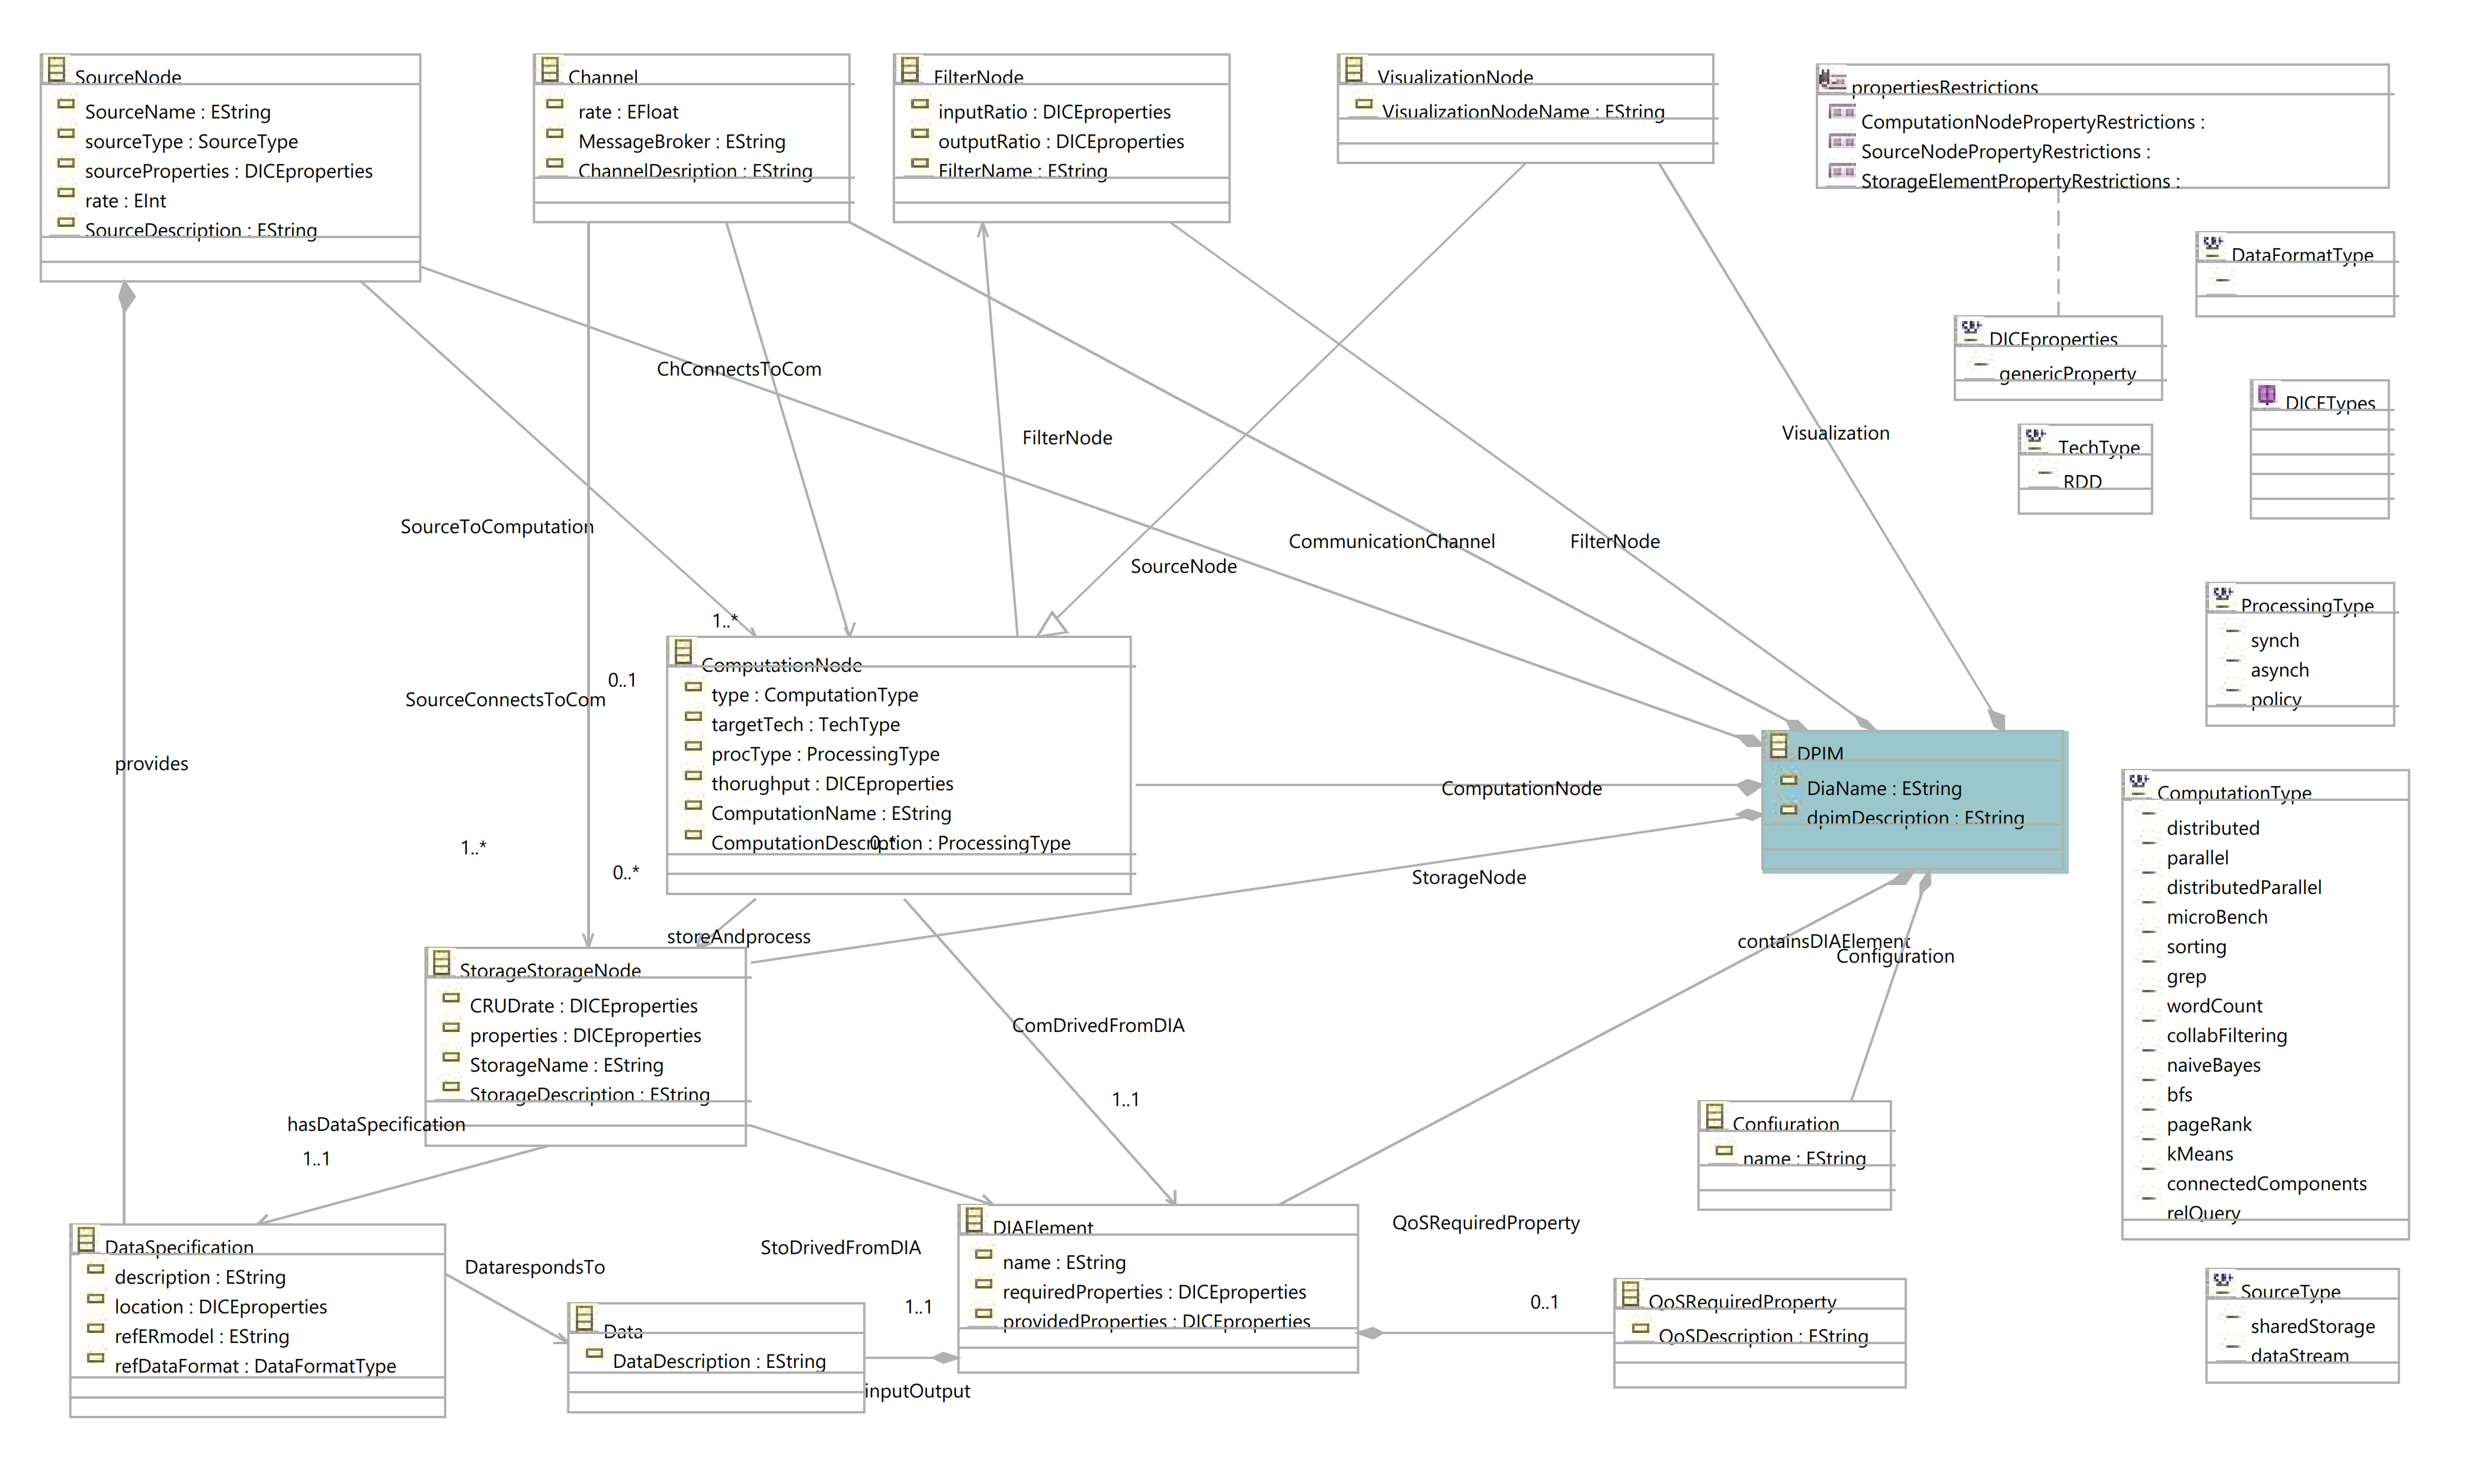
\includegraphics[width=\textwidth]{Images/11.png}
%\caption{\label{fig:metamodel}DICE DPIM metamodel.}
%\end{sidewaysfigure}

%\begin{figure}
%\centering
%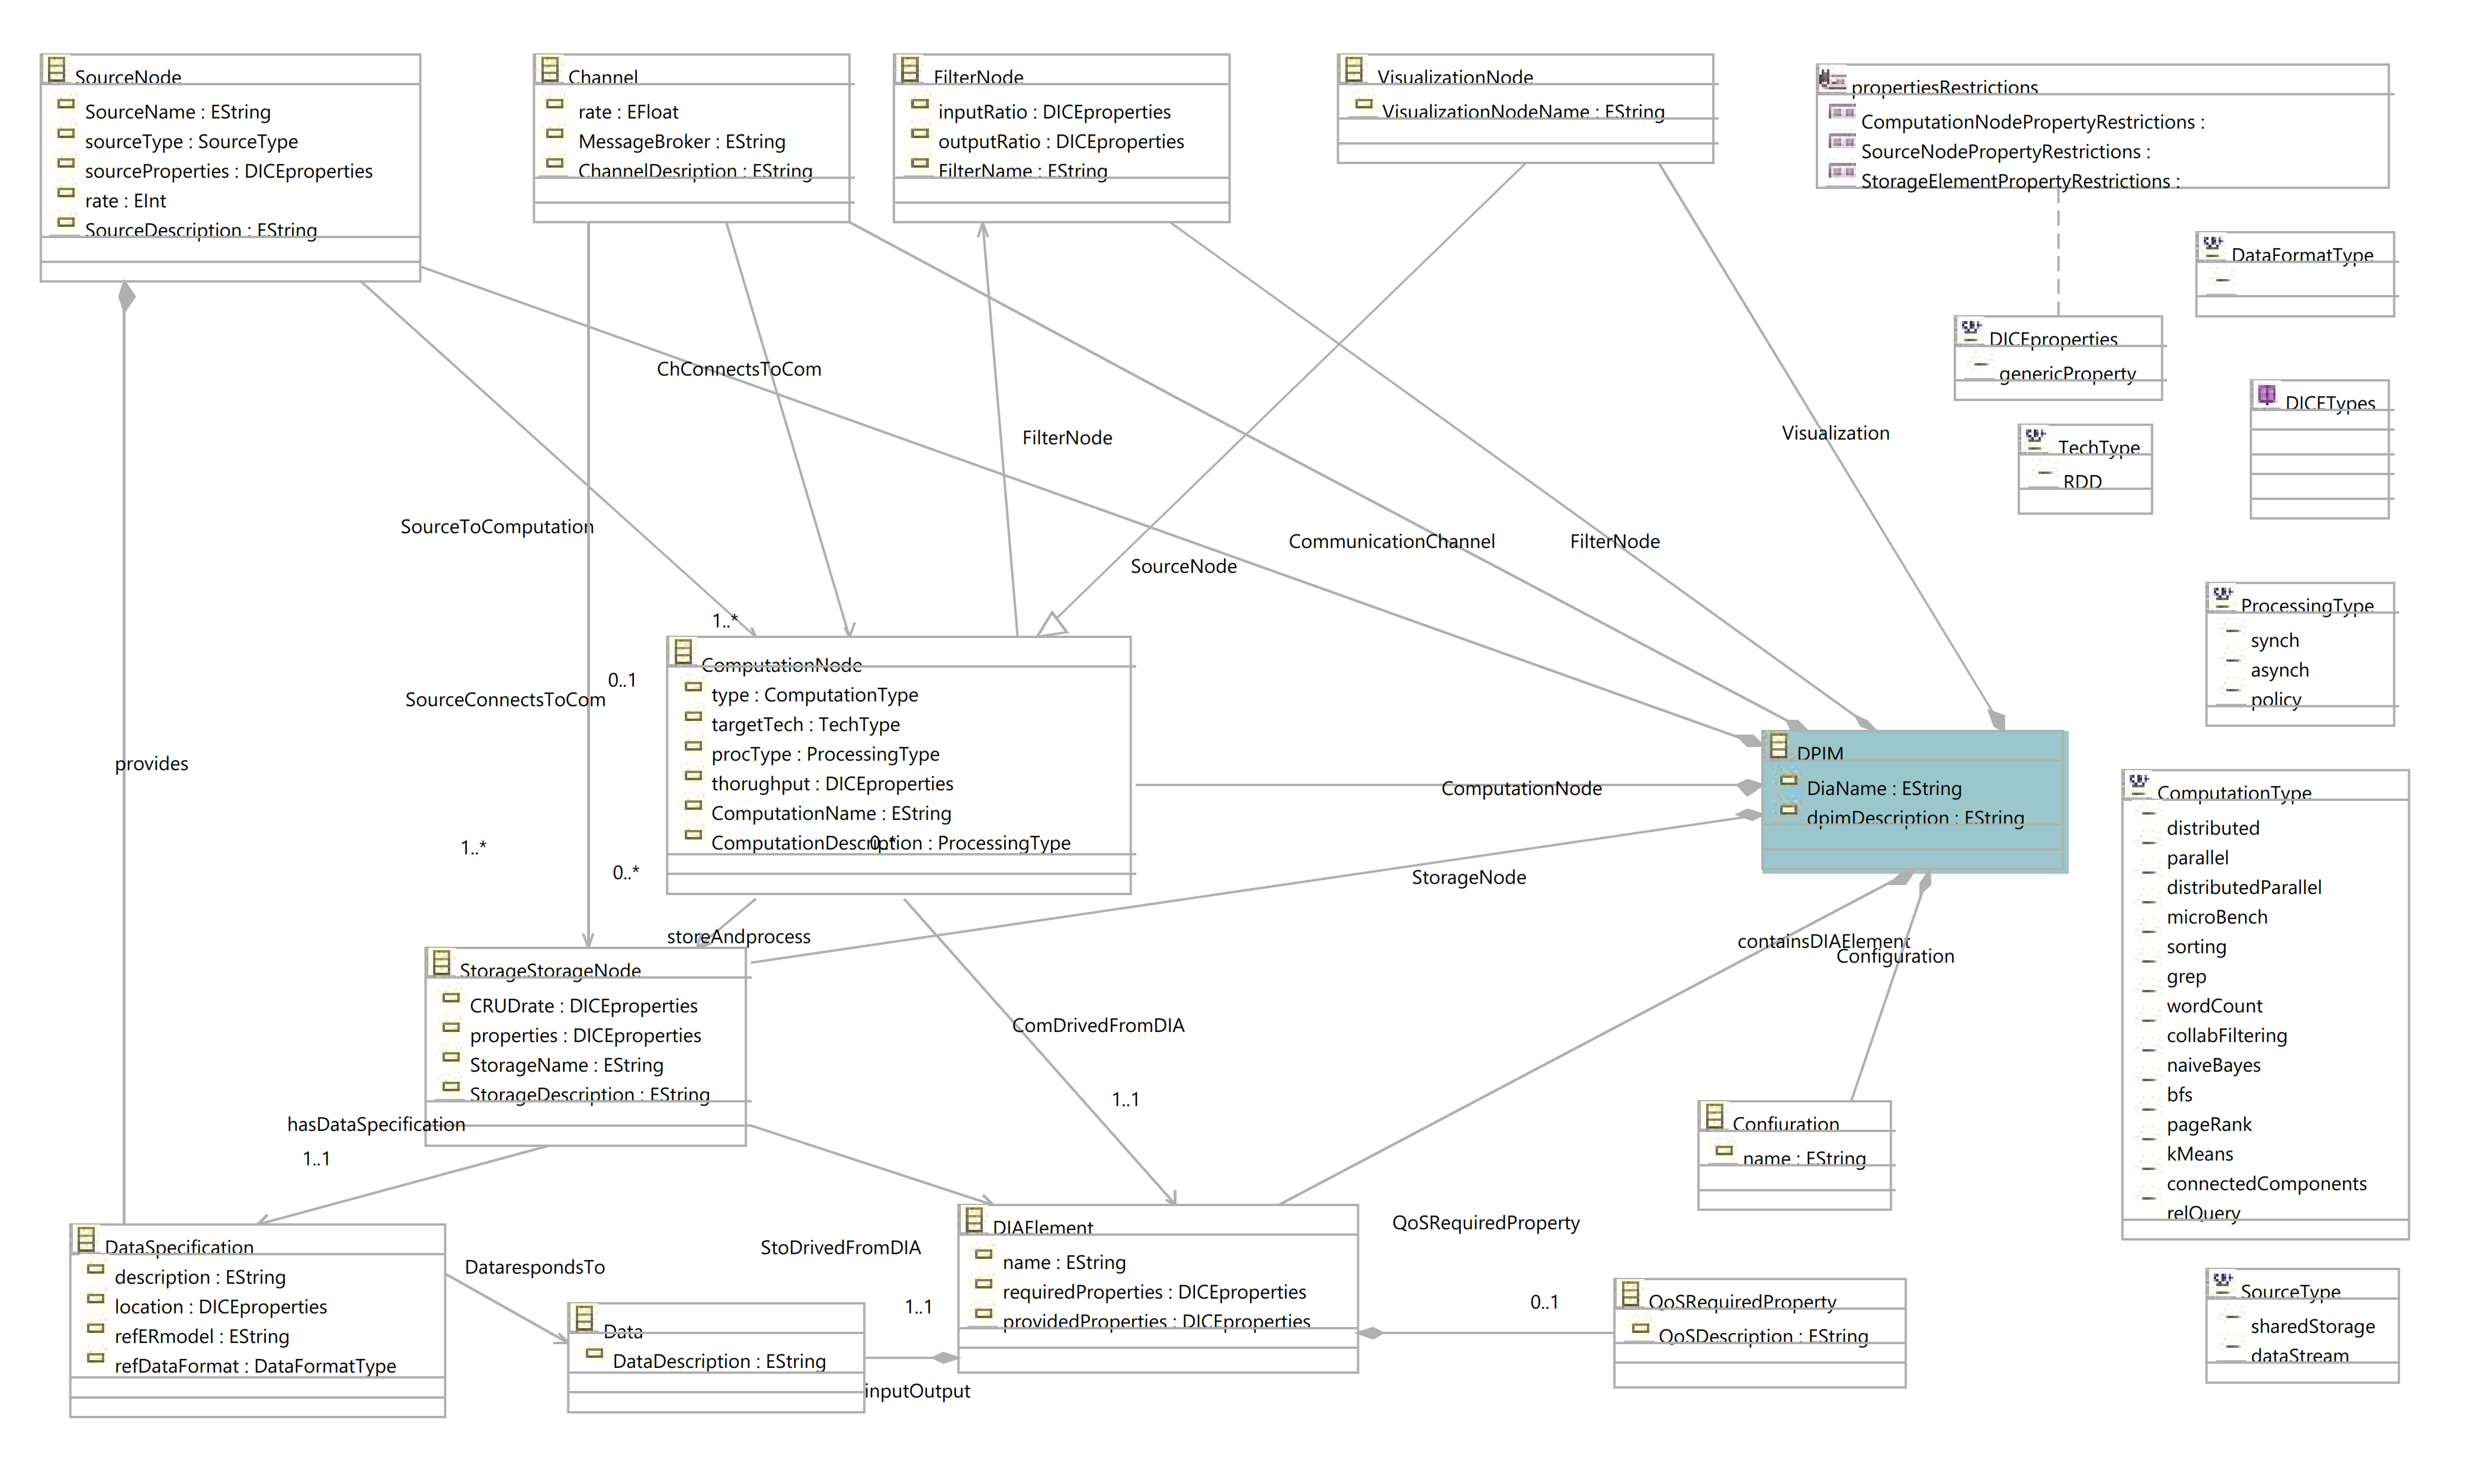
\includegraphics[width=\textwidth]{Images/11.png}
%\caption{\label{fig:metamodel2}DICE DPIM metamodel in portrait form.}
%\end{figure}

\subsection{Scenarios}
\label{subsect:scenarios}

We want to start this section presenting some usefull scenarios in order to describe what people will do and experience as they try to make use of CLup services. Our intent is not to specify every possible situation, but to give the reader a general understanding of the main features of the system with a concrete description of ideal cases.
 
\begin{description}
    \item[User lines up] 
    %In a period of global pandemic and quarantine, XXX needs to do the grocery shopping and, remembering the risks he used to take when there was no organization, he smiles opening the CLup app from his smartphone. He immediately searches the store he wants to go to, and in a few clicks he has all the relevant information about the status of the virtual queue and an estimation of how much time to wait. He decides to enqueue himself and by informing the app about his stay at the shop and how he'll reach it, he's ready to confirm and receive his personal QR code. Now it's time for XXX to wait in the comfort of his house, untill, when the time comes, he receives a push(?) notification from the app telling him that it is the right moment to head towards his destination. When he arrives he finds no queue outside the store, and, by simply scanning his QR code, he's able to enter and exit the shop in a safe and controlled environment.
    Tommy is a student and he’s preparing several exams for the upcoming session.
    He has just now noticed his fridge is empty and he decides to go grocery shopping. Since he needs to study so hard and can't lose any time, he wants to go to the nearest supermarket. He takes out his phone and opens CLup. He immediately looks up for the store he wants to go to and in a few clicks he has himself enqueued! 
    Now it's time for Tommy to wait in the comfort of his house until, when it’s time, he will receive the notification from the app telling him that it is the right moment to head towards his destination. When he arrives he will find no queue outside the store: all time saved up for his studies!


    \item[Customer lines up]
    %As every monday, even this monday Mr. ZZZ goes to the nearby supermarket to gather all he needs for the week. He is used to wait for his turn standing outside in a queue and for someone of his age it's not a simple task. Approaching the entrance of the store he is really surprised noticing that there is no queue, and, rushing inside, he sees a new installation blocking his way: a turnstile and a ticket machine next to it. He reads all the new rules to follow and immediately after he clicked a few button on the new machine, he receives a ticket with the time he needs to wait to enter printed. Now Mr.ZZZ can safely wait his turn while sitting on the benches of the nearby park. When his time will come he'll be able to enter and exit the store scanning the ticket at the turnstile.
    Mrs Sunny would introduce herself as the proud grandmother of three beautiful kids.   
    Every monday, her grandchildren would come visit her, so  Mrs. Sunny goes to the nearby supermarket to gather all she needs for the week. She is used to waiting for her turn standing outside in a queue and for someone of her age it's no simple task to wait on her feet for so long. Approaching the entrance of the store she is really surprised noticing that there is no queue, and, rushing inside, she notices a new installation blocking her way: a turnstile and a ticket machine next to it. She reads all the new rules to follow and, immediately after she clicks a few buttons on the new machine, she receives a ticket that tells her how long she needs to wait to enter and a QR code on it. Now Mrs. Sunny can safely wait his turn while sitting on the bench of the nearby park. 


    \item[User books a visit]
    %YYY has a really strict and rigid work schedule and lately he has found himself unable to go grocery shopping, because of long queues and closing hours of supermarkets. Luckily for him, one of his co-worker tells him that CLup app has a "book a visit" features to better help people manage their time. YYY decides to try it and, after downloading the app and signing up, he searches the store he needs to go to, checks the available reservations, and books the one right after work. The very next day at 7 p.m., when everybody is leaving the office, YYY receives a remainder from the CLup application about his reservation: he will no longer waste a minute in queues neither he'll be left without being able to do the shopping.
    Mr. Zehng  has a really strict and rigid work schedule and lately he has found himself unable to go grocery shopping, because of long queues and closing hours of supermarkets. Luckily for him, one of his co-worker tells him that CLup app has a "book a visit" features to better help people manage their time. Mr. Zehng decides to try it and, after downloading the app and signing up, he looks up for the store he needs to go to, checks the available reservations, and books the one right after work. The very next day at 7 p.m., when everybody is leaving the office, Mr. Zehng receives a reminder from CLup about his reservation: he will no longer waste a minute in queues neither he'll be left without being able to shop.

    \item[Manager registers a shop]
    %During quarantine shops are subjected to strict rule in order to guarantee health safety to their clients. WWW has dealt with a lot of legal problem during the first months of the quarantine, because of how difficult it can be to regulate and monitor traffic through all of his shops. This time he has decided to turn to CLup to precisely regulate the flow of customers and to avoid any problem with crowd forming inside or outside his shops. First of all he visited CLup website and by registering as manager... ?
    Mr. Hochikawa is the owner of a chain of supermarkets.
    During quarantine, shops are subjected to strict rules in order to guarantee health safety to their clients. Indeed, Mr. Hochikawa has been facing a lot of difficulties lately because of how hard it can be to regulate and monitor traffic through all of his shops. Now he has decided to turn to CLup to precisely regulate the flow of customers and to avoid any problem of people crowding up inside and outside his shops. Since when he have had all of his shops registered, it has become just a question of a click to monitor the ones he wants whenever he wants to.\\ Mr. Hochikawa’s life is so much easier now, thanks to Clup.


    \item[Manager updates shop's info]
    %The pandemic is unpredictable and therefore sometimes WWW finds himself having to close his supermarket, or changing some parameters because of new laws. CLup helps him customize everything he needs to, in fact in a few clicks from the app a shop manager can update all the shop's info. For example when… ?
    Miss Lebon owns a little grocery shop downtown and she only sells organic products. Because of this, her product are always very fresh but perish very quickly too. Indeed, she spends much effort in continusly provide her store with new goods. Moreover, the fact that her grocery store is very little, make it very important for her to optimaze the influx of incoming people in her shop. Nethertheless, the fact that she knows with little notice what she will be selling the day after, make it hard for her to organize her store in fixed areas. Thanks to Clup updating function, she can reorganize the areas everyday and make the best out of her sellings. Moreover, with her health food, she helps us make her customers ever healthier!
\end{description}

These scenarios presented highlight the main functions of CLup:
\begin{itemize}[topsep=0pt]
    \item \textit{User/customer lines up};
    \item \textit{User books a visit};
    \item \textit{Manager registers a shop};
\end{itemize}

In addition to these main functions our application has several more features, some supporting the main ones and some essential by themselves, here we list the most notable ones:
\begin{itemize}[topsep=0pt]
    \item \textit{Account registration};
    \item \textit{Users retrieves informations about shops' status};
    \item \textit{Users retrieves informations about booked visits};
    \item \textit{Users retrieves informations about current enqueuements};
    \item \textit{Manager updates shops' information};
    \item \textit{User/cusotmer cancels previous enqueuement or booked visit};
\end{itemize}

Now that the reader has a good understanding of the typical scenarios in wich our application is involved, we'll dig in a more in-depth analysis.

\subsection{Goals}
\label{subsect:goals}

The following tables show in details all the main goals that our application wants to meet. 

We managed to divide them in two main categories: goals related to the shop owners and goals related to the clients. Also, we have assigned an unique identifier to each one of them in order to be able to refer to them later in the document.

\begin{table}[h!]
    \centering
    \begin{tabular}{@{}P{0.1\textwidth}P{0.80\textwidth}@{}}
        \multicolumn{2}{c}{\textbf{Shop owners}} \\
        \toprule
        \textbf{Identifier}& \textbf{Goal}\\
        \midrule
        \textbf{G1}        & Allow manager to sign on the system\\
        \textbf{G2}        & Allow a manager to sign in the system\\
        \textbf{G3}        & Allow a manager to register their store/stores on the system\\
        $\;\;$    G3.1  & Allow a manager to register basic info about the shop\\
        $\;\;$    G3.2  & Allow a manager to divide their store in areas \\
        $\;\;$    G3.3  & Allow a manager to register the items in the areas \\
        \textbf{G4}        & Allow a manager to update the shop's informations and settings\\
        \textbf{G5}        & Allow a manager to check the general status of their shop\\
        \textbf{G6}        & Allow a manager to cancel a previously booked shopping session for an user \\
        \textbf{G7}        & TODO: The system should be accessible to all kind of users and customers\\
    \end{tabular}
\caption{Shop owner's goals}
\label{table:shopownersgoals}
\end{table}

\begin{table}[h!]
    \centering
    \begin{tabular}{@{}P{0.1\textwidth}P{0.80\textwidth}@{}}
        \multicolumn{2}{c}{\textbf{Clients}} \\
        \toprule
        \textbf{Identifier}& \textbf{Goal}\\
        \midrule
        \textbf{G8}        & Allow a customer to join a virtual queue from the spot\footnotemark[1]\\
        \textbf{G9}        & Allow a user to sign on the system\\
        \textbf{G10}       & Allow a user to sign in the system\\
        \textbf{G11}       & Allow a user to join the virtual queue from the app or website\\
        \textbf{G12}       & Allow a user to book a shopping session at a grocery store\\
        $\;\;$    G12.1 & Allow a user to select the time and duration for they session\\ 	
        $\;\;$    G12.2 & Allow a user to select categories of items they are willing to buy\\
        \textbf{G13}       & Allow a user to retrieve informations about its previously booked visits\\
        \textbf{G14}       & Allaw a user to retrieve informations about current enqueuements\\
        \textbf{G15}       & Allow a user to retrieve informations about shops\\
        \textbf{G16}       & Allow a users and customers to enter and exit stores with QR codes\\
        \textbf{G17}       & Allow a user to exit a previously joined queue \\
        \textbf{G18}       & Allow customers to line up\footnotemark[2]\\
        \textbf{G19}       & Allow a customer to cancel a previously booked visit \\
        \textbf{G20}       & Allow a user to cancel a previously booked visit\footnotemark[1] \\

        \bottomrule
    \end{tabular}
\caption{Client's goals}
\label{table:clientsgoals}
\end{table}
\footnotetext[1]{with the facility of a hardware support, it will be better specificed later on this document.}
\footnotetext[2]{to the customer's eyes it seems like an enqueuement, but from the system perspective the entire process is handled as a booked visits, it will be better specified later on this document.}

\FloatBarrier

\subsection{Domain Assumptions}
\label{subsect:domainassumptions}

The following table lists all the assumptions over which we cannot have control, but we assume as verified.

As with the goals in the section above, we provide them with an unique identifier to keep track of them in the document.

TODO: what abaout multiple enqueuement?? and what about overlapping visits? we have not specified anything about it! Also only one reservation in one shop.

TODO: questione degli stati del ticket: unavailable (prima di poter essere usato), available (quando può essere usato), inuse/active (quando lo si sta usando), expired/used (quando è scaduto o è finito di essere usato, magari questo può combaciare con unavailable, ma per una questione di rappresentazione degli stati eviterei)

TODO: introducing an administrator account to add shops.

\begin{table}[h!]
    \centering
    \begin{tabular}{@{}P{0.1\textwidth}P{0.80\textwidth}@{}}
        \toprule
        \textbf{identifier}& \textbf{Domain Assumption}\\
        \midrule
        \textbf{D1}        & Data provided from GPS is valid and accurate TODO: non dovremmo dire quanto accurato?\\
        \textbf{D2}        & Google Maps' paths calculator makes correct time estimations\\
        \textbf{D3}        & A person cannot get in the store without having scanned the QR code\\
        \textbf{D4}        & A person cannot get out of the store without having scanned the QR code\\
        \textbf{D5}        & Each store registered on the system is provided with the necessary functioning hardware\\
        \textbf{D6}        & Data provided from managers is legit\\
        $\;\;$D6.1         & Managers provide the maximum number of person allowed in the store by the law\\
        $\;\;$D6.2         & Managers will provide the correct address of their store\\
        $\;\;$D6.3         & Managers will provide the correct schedule of their store\\
        $\;\;$D6.4         & Managers will provide the correct categories of items they sell\\
        $\;\;$D6.5         & Managers will correctly map items with the respective category\\
        \textbf{D7}        & Every category of a shop is matched with an area non overlapping with any other categories' area\\
        \textbf{D8}        & A customer will take the shortest path to the store (TODO: non mi convince, perchè in realtà se non lo fanno non me ne frega, che perdano il loro turno questi maledetti! ARGH)\\
        \textbf{D9}        & Customers will stay in the store approximately the time they have claimed they would (TODO: non sono sicuro sia una domain assumption, perchè è una precisazione inaccurata con quel termine "approximately", e inoltre anche se un utente non lo fa non me ne frega, cioè tutti aspettano e amen. DOVREMMO NOTIFICARE IL MANAGER DEL NEGOZIO SE QUALCUNO STA TROPPO DENTRO, IN MODO CHE POSSA O DIRGLI DI ANARSENE, OPPURE MAGARI SE NE E' GIà USCITO SENZA TIMBRARE E QUINDI DI ELIMINARLO DAL NEGOZIO NEL SISTEMA)\\
        \textbf{D10}       & Customers will shop the items they have claimed they would\\
        \textbf{D11}       & Phone numbers are unique\\
        \textbf{D12}       & Emails are unique\\
        \textbf{D13}       & Notification sent to the users, may them be managers or clients, will be received and comprehended by them\\
        \textbf{D14}       & People have no (TODO: si dice così?:) malicious behavior against the app (TODO: well, problem solved. lol... )\\
        \textbf{D15}       & Managers' emails are correctly validated by PEC system (TODO: indagare)\\
        \textbf{D16}       & Users are aware of the process required to scan a QR code\\
        \textbf{D17}       & One QR code scanned means that one and one only person enters the store\\
        \bottomrule
    \end{tabular}
\caption{Domain assumptions}
\label{table:domainassumptions}
\end{table}

\FloatBarrier

\subsection{Constraints}
\label{subsect:contraints}

\subsubsection{Regulatory policies}
\label{subsubsect:regulatorypolicies}

As CLup is an application that deals with real persons' data, it must respect user's privacy and follow strict rules and laws concerning privacy.

Here we show a list of mandatory aspects to consider in order to correctly release an application like CLup:
\begin{itemize}
    \item set rules and protect application's and users' interests with Terms ans Conditions TODO: maybe its a goal??;
    \item ask user permission to retrieve and use GPS data;
    \item regulate cookie management;
    \item telephone numbers and emails will not be used for commercial purpose;
    \item all data about user's booked visits or enqueued clients accessible for statistic's and monitoring purposes is anonymous to the end users.
\end{itemize}

\subsubsection{Hardware limitations}
\label{subsubsect:hardwarelimitations}

In order to reach all kind of users and customers, our application wants to be the most accessible as possible. To achive this goal we intend to release various version of the application for different devices:

\begin{itemize}
    \item \textbf{Mobile app}: Requires a smartphone with internet connection, either Android or Ios. It is not necessary to have GPS to run and use the application, but only to have access to some features.
    \item \textbf{Web app}: Requires a modern browser with javascript enabled and with an internet connection. The capability of retrieving user location is not necessary, but in order to have access to some features is mandatory.
    \item \textbf{Shop's hardware}: Our intent is to have shop owners install hardware facilities that comprehend a totem, a QR scanner and an electronic turnstile. The totem will have internet connection and run a special version of the web application. The QR scanner and electronic turnstile will work togheter to allow access to the stores. 
\end{itemize}

\subsubsection{Interfaces to other applications}
\label{subsubsect:interfacestootherappications}

Our application will rely on external services to handle some features:

\begin{itemize}
    \item GPS TODO: non so se è un interfaccia, anzi penso proprio di no
    \item Google Maps
    \item TODO: LOG IN MANAGEMENT SYSTEM?
\end{itemize}

\subsection{Actors}
\label{subsect:actors}
TODO: io questa sezione la balzerei (è già scritto tutto nelle definition) a meno che non mettiamo un sys admin e così qua lo specifichiamo
\begin{itemize}
    \item user
    \item customer
    \item manager
    \item shop owner
    \item sys admin
\end{itemize}

\subsection{Use cases}
\label{subsect:usecases} 

In this section we want to present all the major activities concerning the interaction between the application and the actors.

We will present a table for each use case and, for the most important ones, a list of sequence diagrams that will cover all the interaction between the actors and the system in a graphical way. For better clarity in the exposure and navigation throught the document we present an organized index of all the use cases with the relatives links to tables and, if present, to sequence diagrams:
\begin{table}[h!]
    \centering
    \begin{tabular}{@{}P{0.57\textwidth}P{0.20\textwidth}P{0.20\textwidth}@{}}
        & \textbf{Description table} & \textbf{Sequence Diagram}\\
        \toprule
        \textbf{1. Customer registration} & tab.\ref{table:customerregitration} & \\
        \textbf{2. shop owner registration} & tab.\ref{table:shopownerregistration} & \\
        \textbf{3. User logs in} & tab.\ref{table:login} & \\
        \textbf{4. Manager logs in} & tab.\ref{table:login} & \\
        \textbf{5. User searches shop}& tab.\ref{table:usersearchesshop} & fig.\ref{fig:usersearchesshop}\\
        \textbf{6. User gets more information} & tab.\ref{table:usergetmoreinformation}& \\
        \textbf{7. User lines up} & tab.\ref{table:userlinesup} & fig.\ref{fig:userlinesup}\\
        \textbf{8. User books a visit} & tab.\ref{table:userbooksavisit} & fig.\ref{fig:userbookavisit}\\
        \textbf{9. Customer lines up} & tab.\ref{table:customerlinesup}& fig.\ref{fig:customerlinesup}\\
        \textbf{10. User/customer enters shop} & tab.\ref{table:entershop} & \\
        \textbf{11. User/customer exits shop} & tab.\ref{table:exitshop} & \\
        \textbf{12. Manager registers new shop} & tab.\ref{table:managerregisternewshop} & \\
        \textbf{13. Manager updates shop's information and settings} & tab.\ref{table:managerupdatesshopinformation} & \\
        \textbf{14. Manager checks shop status} & tab.\ref{table:managerchecksshopstatus} & \\
        \textbf{15. User cancels previously booked visit} & tab.\ref{table:usercancelspreviouslybookedvisit} & \\
        \textbf{16. Customer cancels previously booked visit} & tab.\ref{table:customercnacelspreviousenqueuement} & \\
        \textbf{17. Manager cancels customer's previously booked visit} & tab.\ref{table:managercancelscustomerspreviouslybookedvisit} & \\
        \textbf{18. User cancels previous enqueuement} & tab.\ref{table:usercnacelspreviousenquement} & \\
        \bottomrule
    \end{tabular}
\caption{All use cases}
\label{table:usecase1}
\end{table}

\subsubsection{Use cases tables}

\begin{table}[h!]
    \centering
    \begin{tabular}{@{}P{0.2\textwidth}P{0.70\textwidth}@{}}
        \toprule
        \textbf{Name}                 & Customer registration\\
        \midrule
        \textbf{Actors}               & customer\\
        \textbf{Entry condition}      & the customer is already on the front page of the web or mobile application\\
        \textbf{Flow of events} 
        & i. the customer selects the sign up option\\
        & ii. the customer fills in all of the mandatory fields and then confirms\\
        & iii. the system sends an SMS with a code to the customer's previously specified phone number and waits 180 seconds for an a answer\\
        & iv. the customer validates his phone number by inserting the code\\
        & v. the systems sends an email with a code to the customer's previously specified address and waits 180 seconds for an a answer\\
        & vi. the customer validates his email address by inserting the code\\
        & vii. the system create a new account and redirects the new user to his personal home page\\
        \textbf{Exit condition}       & the customer successfully ends the registration process and becomes a new user\\
        \textbf{Exceptions}           
        & - timer expiration\\
        & - wrong codes\\
        & - email or phone number already registered or not valid\\
        & - the customer insterts not valid informations in one or more mandatory fields\\
        \bottomrule
    \end{tabular}
\caption{Customer registration}
\label{table:customerregitration}
\end{table}

\begin{table}[h!]
    \centering
    \begin{tabular}{@{}P{0.2\textwidth}P{0.70\textwidth}@{}}
        \toprule
        \textbf{Name}                 & Shop owner registration\\
        \midrule
        \textbf{Actors}               & shop owner\\
        \textbf{Entry condition}      & the shop owner is already on the front page of the web or mobile application\\
        \textbf{Flow of events}            
        & i. the shop owner selects the sign up option\\
        & ii. the shop owner specifies he wants to sign up as a manager\\
        & iii. the manager creates a personal private profile filling in all of the mandatory fields such as: name, surname, age, PEC email, telephone number, password, repeat password, \ldots and confirms\\
        & iv. the system sends an SMS with a code to the shop owner's previously specified phone number and waits 180 seconds for an a answer\\
        & v. the shop owner validates his phone number by inserting the code\\
        & vi. the systems sends an email with a code to the shop owner's previously specified address and waits 180 seconds for an a answer\\
        & vii. the shop owner validates his email address by inserting the code\\
        & vii. the system create a new account and redirects the new manager to his personal home page\\
        & viii. TODO\\
        \textbf{Exit condition}       & the shop owner successfully ends the registration process and become a new manager\\
        \textbf{Exceptions}           
        & - timer expiration\\
        & - wrong codes\\
        & - email or phone number already registered or not valid\\
        & - PEC email not verified\\
        & - the customer insterts not valid informations in one or more mandatory fields\\
        \bottomrule
    \end{tabular}
\caption{Shop owner registration}
\label{table:shopownerregistration}
\end{table}

\begin{table}[h!]
    \centering
    \begin{tabular}{@{}P{0.2\textwidth}P{0.70\textwidth}@{}}
        \toprule
        \textbf{Name}                 & User/Manager log in\\
        \midrule
        \textbf{Actors}               & user or manager\\
        \textbf{Entry condition}      & the actor is already on the front page of the web or mobile application\\
        \textbf{Flow of events}            
        & i. the actor selects the sing in option\\
        & ii. the actor compiles the email and password fields and confirms by clicking on the log in button \\
        & iii. the system redirects the actors to the respective home pages\\
        \textbf{Exit condition}       & the actors are successfully redirected to their respective personal home page\\
        \textbf{Exceptions}           
        & - email or password aren’t correct \\
        \bottomrule
    \end{tabular}
\caption{User/Manager log in}
\label{table:login}
\end{table}

\begin{table}[h!]
    \centering
    \begin{tabular}{@{}P{0.2\textwidth}P{0.70\textwidth}@{}}
        \toprule
        \textbf{Name}                 & User searches a shop\\
        \midrule
        \textbf{Actors}               & user\\
        \textbf{Entry condition}      & user logged in and on his web or mobile personal home page\\
        \textbf{Flow of events}            
        & i. user selects the search a shop option\\
        & ii. the system gets the user's position using GPS and after retrieving the shops adhering to CLups near him, shows them in a map and, also, in a list\\
        & iii. the user either types the name of the shop they want to find in the search bar or navigates the map or scrolls the list\\
        & iv. the user selects a shop\\
        & v. the application retrieves all the necessary information about the selected shop's status and information, displays them to the user with the list of possible action the user can take: book a visit or enqueue or get more info\\
        \textbf{Exit condition}       & the user successfully finds the shop he was looking for\\
        \textbf{Exceptions}           
        & - the shop searched doesn't exists or isn't adhering to CLup\\
        & - GPS is off\\
        \textbf{Notes} & an user searches for a shop in order to get general informations or check its status or to enqueue himself or to book a visit\\
        \bottomrule
    \end{tabular}
\caption{User searches a shop}
\label{table:usersearchesshop}
\end{table}

\begin{table}[h!]
    \centering
    \begin{tabular}{@{}P{0.2\textwidth}P{0.70\textwidth}@{}}
        \toprule
        \textbf{Name}                 & User gets more information\\
        \midrule
        \textbf{Actors}               & user\\
        \textbf{Entry condition}      & the user is successfully at the exit condition of "user searches a shop" use case (table \ref{table:usersearchesshop})\\
        \textbf{Flow of events}            
        & i. the user selects the get more info option\\
        & ii. the system retrieves further details about the shop and displays them to the user\\
        & iii. the user visualizes the informations\\
        \textbf{Exit condition}       & the user can visualize the information needed\\
        \bottomrule
    \end{tabular}
\caption{User gets more information}
\label{table:usergetmoreinformation}
\end{table}

\begin{table}[h!]
    \centering
    \begin{tabular}{@{}P{0.2\textwidth}P{0.70\textwidth}@{}}
        \toprule
        \textbf{Name}                 & User lines up\\
        \midrule
        \textbf{Actors}               & user\\
        \textbf{Entry condition}      & the user is successfully at the exit condition of "user searches a shop" use case (table \ref{table:usersearchesshop})\\
        \textbf{Flow of events}            
        & i. the user selects the line up option\\
        & ii. the user specifies the estimated time he thinks he will spend at the shop\\
        & iii. optionally the user either activates GPS and specifies by what mean they are going to reach the shop or specifies how much time he needs to reach the shop\\
        & iv. if the store has divided his store in categories, the user can optionally specify what categories he is interested in\\
        & v. the system adds the user to the queue and displays a constantly updated page with all the relevant information about the enqueuement\\
        \textbf{Exit condition}       & the user is correctly enqueued and needs to wait for his turn\\
        \textbf{Exceptions}           
        & - the enqueuement is not possible\\ %some weird and really really edge cases of simmultaneus enqueuement
        & - GPS is not active\\
        \textbf{Notes} & the page with all the enqueuement information can be also reached by the user at any moment from his personal home page when he is currently enqueued\\
        \bottomrule
    \end{tabular}
\caption{User lines up}
\label{table:userlinesup}
\end{table}

\begin{table}[h!]
    \centering
    \begin{tabular}{@{}P{0.2\textwidth}P{0.70\textwidth}@{}}
        \toprule
        \textbf{Name}                 & User books a visit\\
        \midrule
        \textbf{Actors}               & user\\
        \textbf{Entry condition}      & the user is successfully at the exit condition of "user searches a shop" use case (table \ref{table:usersearchesshop})\\
        \textbf{Flow of events}            
        & i. the user selects the book a visit option\\
        & ii. the user specifies the estimated time he thinks he will spend at the shop\\
        & iii. if the store has divided his store in categories, the user can optionally specify what categories he is interested in\\
        & iv. the system retrieves the possible slots and displays the options to the user\\
        & v. the user chooses the slots he prefers and confirms\\
        & vi. the system registers the visit, sends confirmation to the user and redirects him to a page with all the relevant infromation about the booked visit\\
        \textbf{Exit condition}       & the user has correctly booked a visit\\
        \textbf{Exceptions}           
        & - the reservation is not possible\\
        & - the user can't find any available slot\\
        \textbf{Notes} 
        & -the order of the various information requested to the user is important in order to let the system decide what possible slots are available\\
        & -The page with all relevant information about the visit is easily accessible: from the user's personal home page there's an option to check all the reservation, this option leads to a page with all the reservations and by selecting one the user can reach the said page\\
        \bottomrule
    \end{tabular}
\caption{User books a visit}
\label{table:userbooksavisit}
\end{table}

\begin{table}[h!]
    \centering
    \begin{tabular}{@{}P{0.2\textwidth}P{0.70\textwidth}@{}}
        \toprule
        \textbf{Name}                 & Customer lines up\\
        \midrule
        \textbf{Actors}               & customer\\
        \textbf{Entry condition}      & the customer is at the entrance of the hop and have read and understood the functioning of the hardware\\
        \textbf{Flow of events}            
        & i. the customer visualize information about the status of the shop\\
        & ii. the customer select the enqueue option on the totem\\
        & iii. the customer specifies the estimated time he thinks he will spend at the shop\\
        & iv. the system books a visit for the customer at the first available slot\\
        & v. the totem retrieves the visit's information and prints a ticket with them\\
        & vi. the customer takes the ticket\\
        \textbf{Exit condition}       & the cusotmer succesfully retrieves his ticket and has a booked visit registered\\
        \textbf{Exceptions}           
        & - enqueuement is not possible\\
        & - hardaware is not functioning properly\\
        \bottomrule
    \end{tabular}
\caption{Customer lines up}
\label{table:customerlinesup}
\end{table}

\begin{table}[h!]
    \centering
    \begin{tabular}{@{}P{0.2\textwidth}P{0.70\textwidth}@{}}
        \toprule
        \textbf{Name}                 & User/customer enters the shop\\
        \midrule
        \textbf{Actors}               & user, customer\\
        \textbf{Entry condition}      & have previously enqueued or have previously booked a visit\\
        \textbf{Flow of events}            
        & i. the actor arrives at the shop\\
        & ii. the actor correctly places the QR code on the QR code scanner facility at the entrance of the shop\\
        & iii. the system correctly scans the QR code\\
        & iv. the system unlocks the turnstile\\
        & v. the actor enters the shop\\
        \textbf{Exit condition}       & the user/customer get inside the shop\\
        \textbf{Exceptions}           
        & - the QR code is not valid\\
        & - the hardware is not functioning properly\\
        \bottomrule
    \end{tabular}
\caption{}
\label{table:entershop}
\end{table}

\begin{table}[h!]
    \centering
    \begin{tabular}{@{}P{0.2\textwidth}P{0.70\textwidth}@{}}
        \toprule
        \textbf{Name}                 & User/customer exits the shop\\
        \midrule
        \textbf{Actors}               & user, customer\\
        \textbf{Entry condition}      & have previously entered the store with a QR code\\
        \textbf{Flow of events}            
        & i. the actor arrives at the exit of the shop\\
        & ii. the actor correctly places the QR code on the QR code scanner facility at the exit of the shop\\
        & iii. the system correctly scans the QR code\\
        & iv. the system unlocks the turnstile\\
        & v. the actor exit the shop\\
        \textbf{Exit condition}       & the user/customer get out of the shop\\
        \textbf{Exceptions}           
        & - the QR code is not valid\\
        & - the hardware is not functioning properly\\
        \bottomrule
    \end{tabular}
\caption{User/customer exits the shop}
\label{table:exitshop}
\end{table}

\begin{table}[h!]
    \centering
    \begin{tabular}{@{}P{0.2\textwidth}P{0.70\textwidth}@{}}
        \toprule
        \textbf{Name}                 & Manager registers new shop\\
        \midrule
        \textbf{Actors}               & manager logged in and on his web or mobile personal home page\\
        \textbf{Entry condition}      & \\
        \textbf{Flow of events}            
        & i. the manager select the “REGISTER A NEW SHOP” option on the home page, a page pops up with a form to be filled in\\
        & ii.  the manager fills in the mandatory fields (position of the shop, schedule of the shop, opening days, name of the shop, maximum number of people allowed in the shop, optionally the items sold in the shop divided in categories or, for semplicity, just the categories)\\
        & iii. the manager submit the data inserted\\
        & iv. the system correctly registers the shop\\
        & v.the system sends confirmation to the manager\\
        \textbf{Exit condition}       & the shop has been correctly registered\\
        \textbf{Exceptions}           
        & - any of the data inserted in the mandatory fields is invalid\\
        \bottomrule
    \end{tabular}
\caption{Manager registers new shop}
\label{table:managerregisternewshop}
\end{table}

\begin{table}[h!]
    \centering
    \begin{tabular}{@{}P{0.2\textwidth}P{0.70\textwidth}@{}}
        \toprule
        \textbf{Name}                 & Manager updates shop's information and settings\\
        \midrule
        \textbf{Actors}               & manager\\
        \textbf{Entry condition}      & manager logged in and on his web or mobile personal home page\\
        \textbf{Flow of events}            
        & i. the manager selects the update shop info option\\
        & ii. the system redirects the manager to a dedicated page showing all the editable informations and settings\\
        & iii. the manager selects the desired iformation or setting to updadte\\
        & iv. the manager modifies the selected information or settings\\
        & v. the manager confirms the update\\
        & vi. the system updates the shop info\\
        & vii. the system sends confirmation to the manager\\
        \textbf{Exit condition}       & the shop informations or settings are correctly modified\\
        \textbf{Exceptions}           
        & - some new information or setting inserted from the manager is invalid\\
        \bottomrule
    \end{tabular}
\caption{Manager updates shop information}
\label{table:managerupdatesshopinformation}
\end{table}

\begin{table}[h!]
    \centering
    \begin{tabular}{@{}P{0.2\textwidth}P{0.70\textwidth}@{}}
        \toprule
        \textbf{Name}                 & Manager checks shop status\\
        \midrule
        \textbf{Actors}               & manager\\
        \textbf{Entry condition}      & manager logged in and on his web or mobile personal home page\\
        \textbf{Flow of events}            
        & i. the manager selects the check shop status option\\
        & ii. the system retrieves all the informations about the shop and displays them to the manager (number of people actually inside the shop, number of people enqueued, estimated time of enqueuement, upcoming booked visits, etc)\\
        & iii. the manager correctly visualizes such informations\\
        \textbf{Exit condition}       & the manager correctly visualizes the shop status\\
        \bottomrule
    \end{tabular}
\caption{Manager checks shop status}
\label{table:managerchecksshopstatus}
\end{table}

\begin{table}[h!]
    \centering
    \begin{tabular}{@{}P{0.2\textwidth}P{0.70\textwidth}@{}}
        \toprule
        \textbf{Name}                 & User cancels previously booked visit\\
        \midrule
        \textbf{Actors}               & user\\
        \textbf{Entry condition}      & user logged in, on his web or mobile personal home page\\
        \textbf{Flow of events}            
        & i. the user selectes on the check previously booked visits option\\
        & ii. the system retrieves the user's previously booked visits\\
        & iii. the user selects one of his previously booked visits\\
        & iv. the user selects the cancel prenotation option\\
        & v. the system cancels the booked visit and notifies the user of success\\
        \textbf{Exit condition}       & the user successfully canceles the visit\\
        \textbf{Exceptions}           
        & - user has no previously booked visits\\
        \bottomrule
    \end{tabular}
\caption{User cancels previously booked visit}
\label{table:usercancelspreviouslybookedvisit}
\end{table}

\begin{table}[h!]
    \centering
    \begin{tabular}{@{}P{0.2\textwidth}P{0.70\textwidth}@{}}
        \toprule
        \textbf{Name}                 & Customer cancels previous enqueuement\\
        \midrule
        \textbf{Actors}               & customer\\
        \textbf{Entry condition}      & customer infront of the a shop totem that is displaying his home page\\
        \textbf{Flow of events}            
        & i. the customer selects the cancel a booked visit option\\
        & ii. the user insterts the code on his ticket\\
        & iii. the system cancels the booked visit and notifies the customer of success\\
        \textbf{Exit condition}       & the customer successfully cancels his enqueument\\
        \textbf{Exceptions}           
        & - the customer has no booked visit\\
        & - the customer uses the ticket from an already elapsed visit\\
        \bottomrule
    \end{tabular}
\caption{Customer cancels previously enqueuement}
\label{table:customercnacelspreviousenqueuement}
\end{table}

\begin{table}[h!]
    \centering
    \begin{tabular}{@{}P{0.2\textwidth}P{0.70\textwidth}@{}}
        \toprule
        \textbf{Name}                 & Manager cancels customer’s previously booked visit ????? TODO: io la toglierei\\
        \midrule
        \textbf{Actors}               & manager\\
        \textbf{Entry condition}      & the manager is logged in and on his web or mobile personal home page\\
        \textbf{Flow of events}            
        & i. manager PRESS the CHECK PREVIOUSLY BOOKED VISITS button \\
        & ii. the system ask the user to insert a serial number to retrieve the desiderd booked visit\\
        & iii. the manager insert the serial number\\
        & iv. the system cancel the booked visit and notifies the user of the success of action\\
        \textbf{Exit condition}       & the booked visit is successfully canceled\\
        \textbf{Exceptions}           
        & -\\
        \bottomrule
    \end{tabular}
\caption{Manager cancels customer’s previously booked visit}
\label{table:managercancelscustomerspreviouslybookedvisit}
\end{table}

\begin{table}[h!]
    \centering
    \begin{tabular}{@{}P{0.2\textwidth}P{0.70\textwidth}@{}}
        \toprule
        \textbf{Name}                 & User cancels previous enqueuement\\
        \midrule
        \textbf{Entry condition}      & user logged in, on his web or mobile personal home page\\
        \textbf{Flow of events}            
        & i. the user selects the virtual ticket in his home page\\
        & ii. the system retrieves and displays all the information about the ticket and the queue\\
        & iii. the user selects the dequeue button\\
        & iv. the system correctly dequeue the user and notifies the user of success\\
        & v. the system notifies all the user that changed position in the queue\\
        \textbf{Exit condition}       & the user successfully cancels the visit\\
        \textbf{Exceptions}           
        & - the user is not enqueued\\
        \bottomrule
    \end{tabular}
\caption{User cancels previous enqueuement}
\label{table:usercnacelspreviousenquement}
\end{table}

\clearpage

\subsubsection{Use cases sequence diagrams}

\begin{figure}[h!]
    \centering
    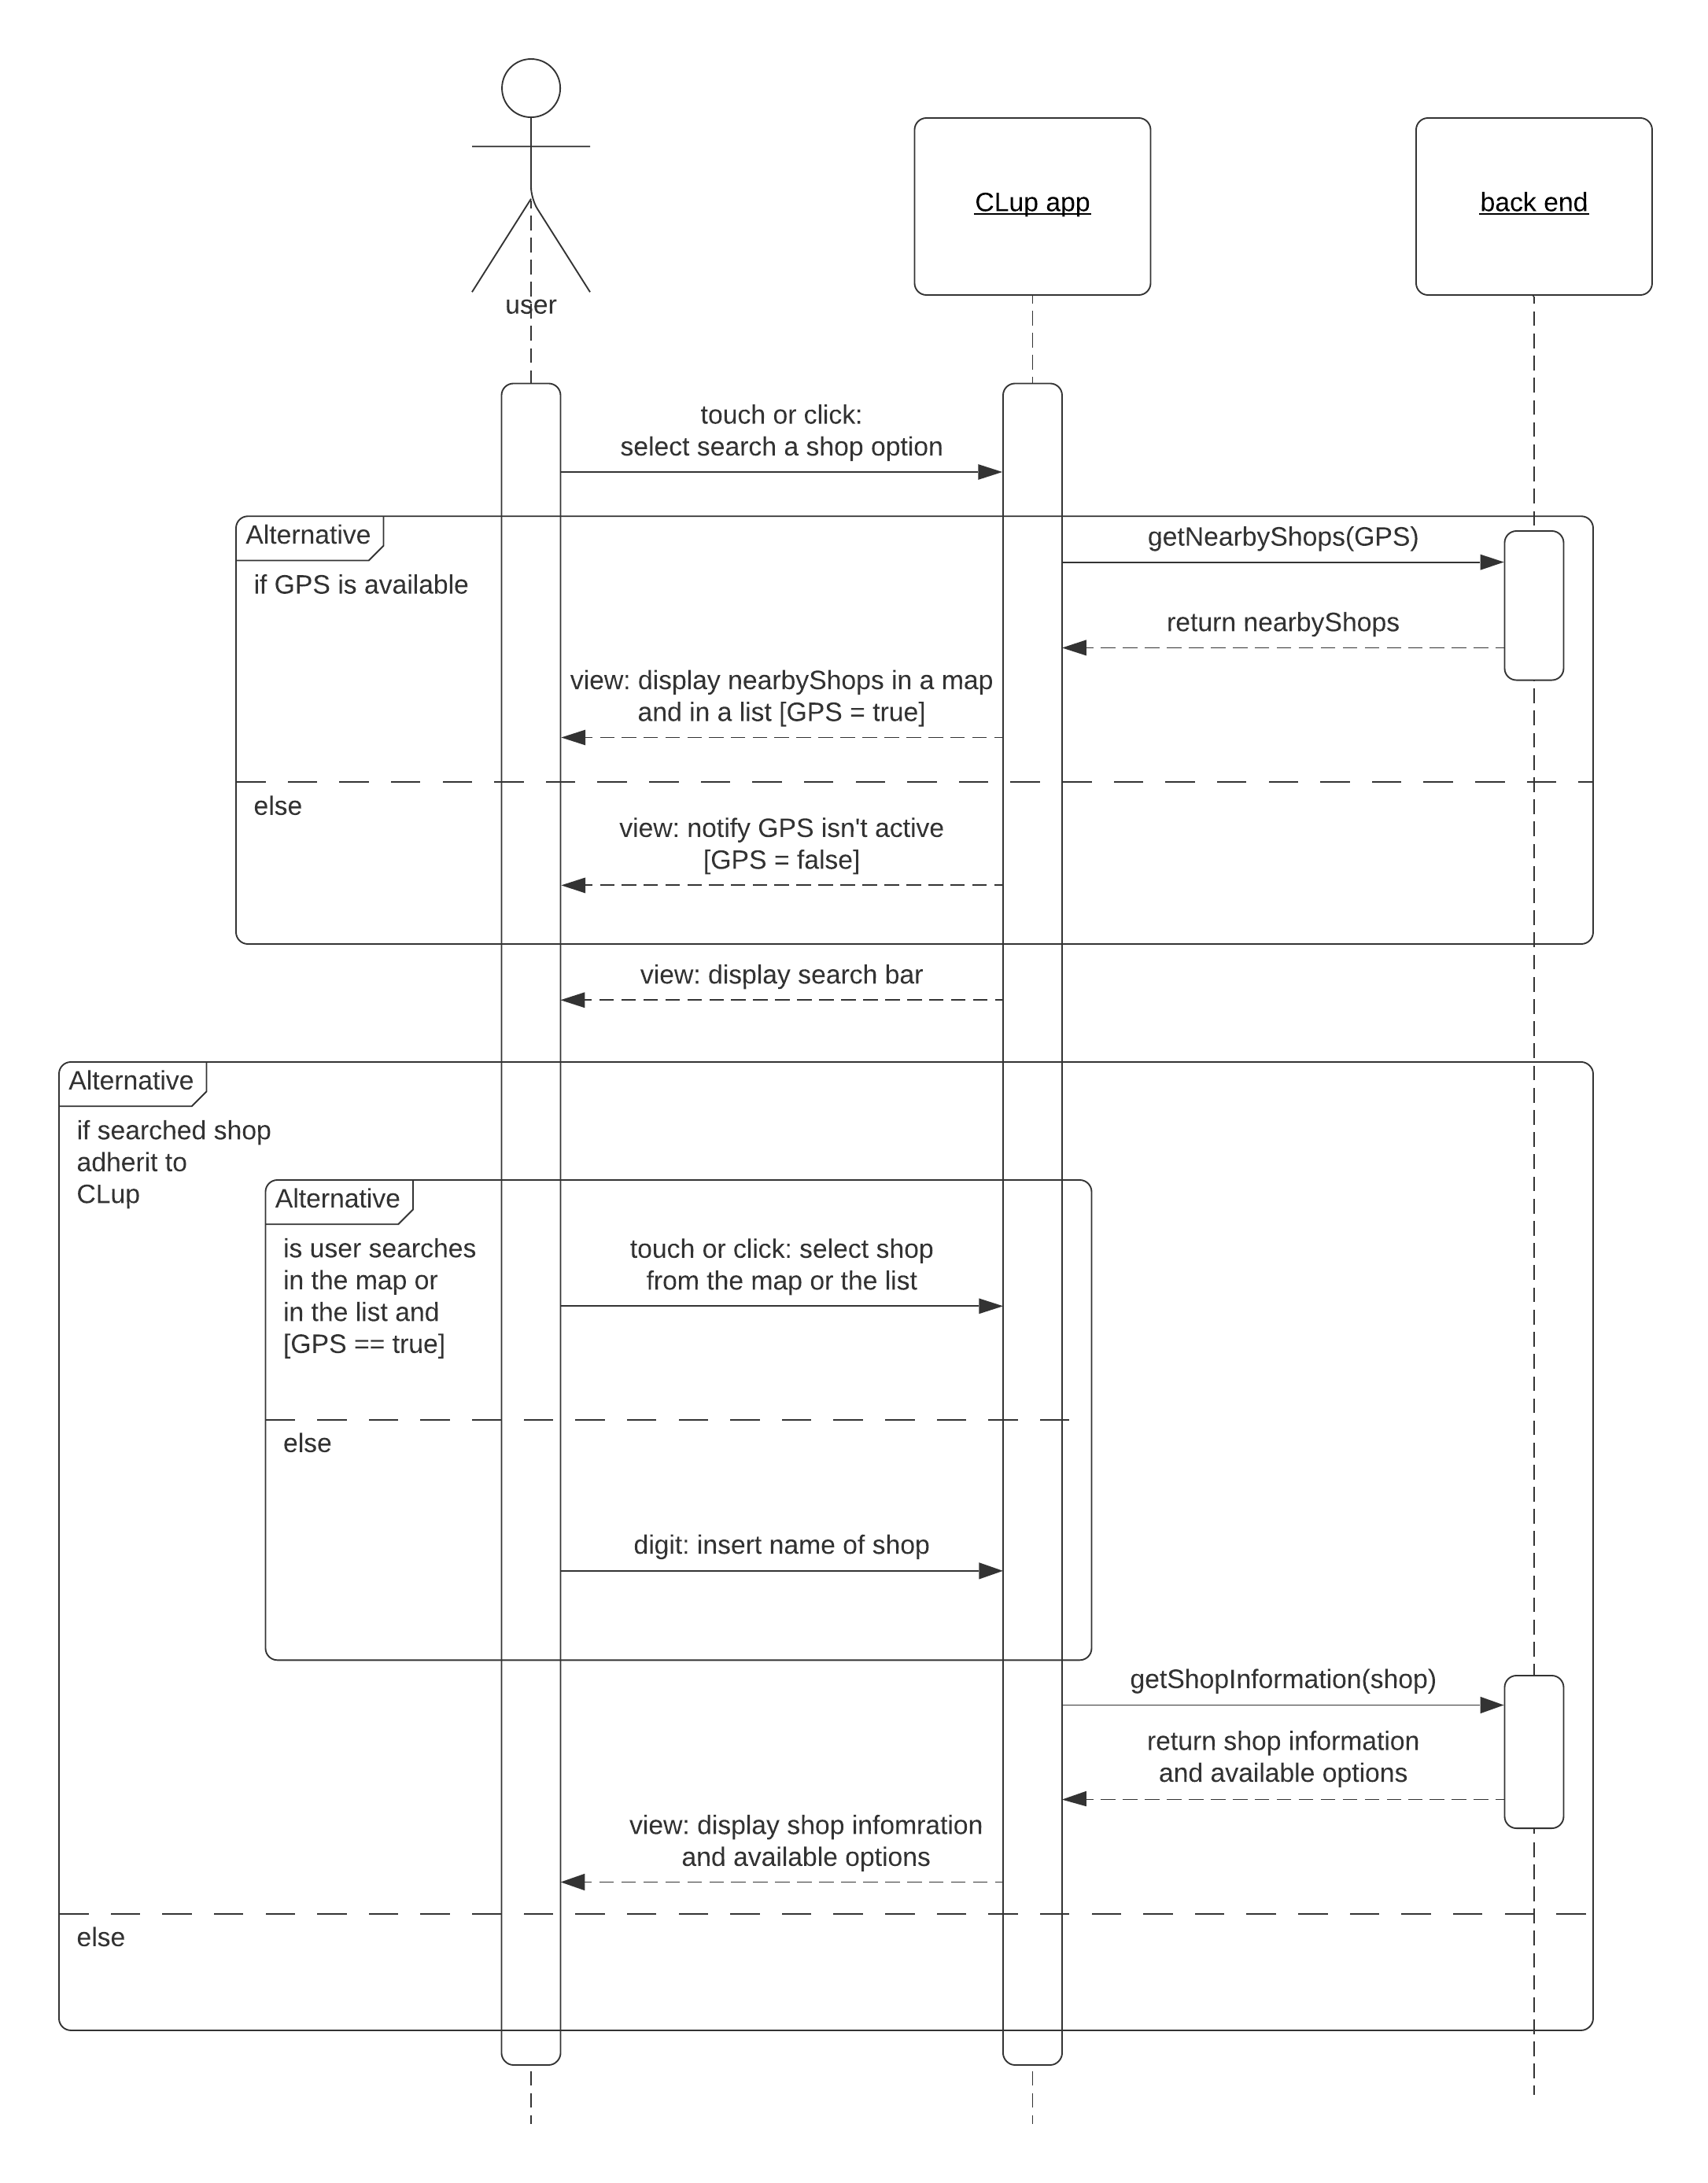
\includegraphics[width=\textwidth]{Images/sequencediagrams/UsersearchesashopSD.png}
    \caption{\label{fig:usersearchesshop}User searches a shop - sequence diagram}
\end{figure}

\begin{figure}[h!]
    \centering
    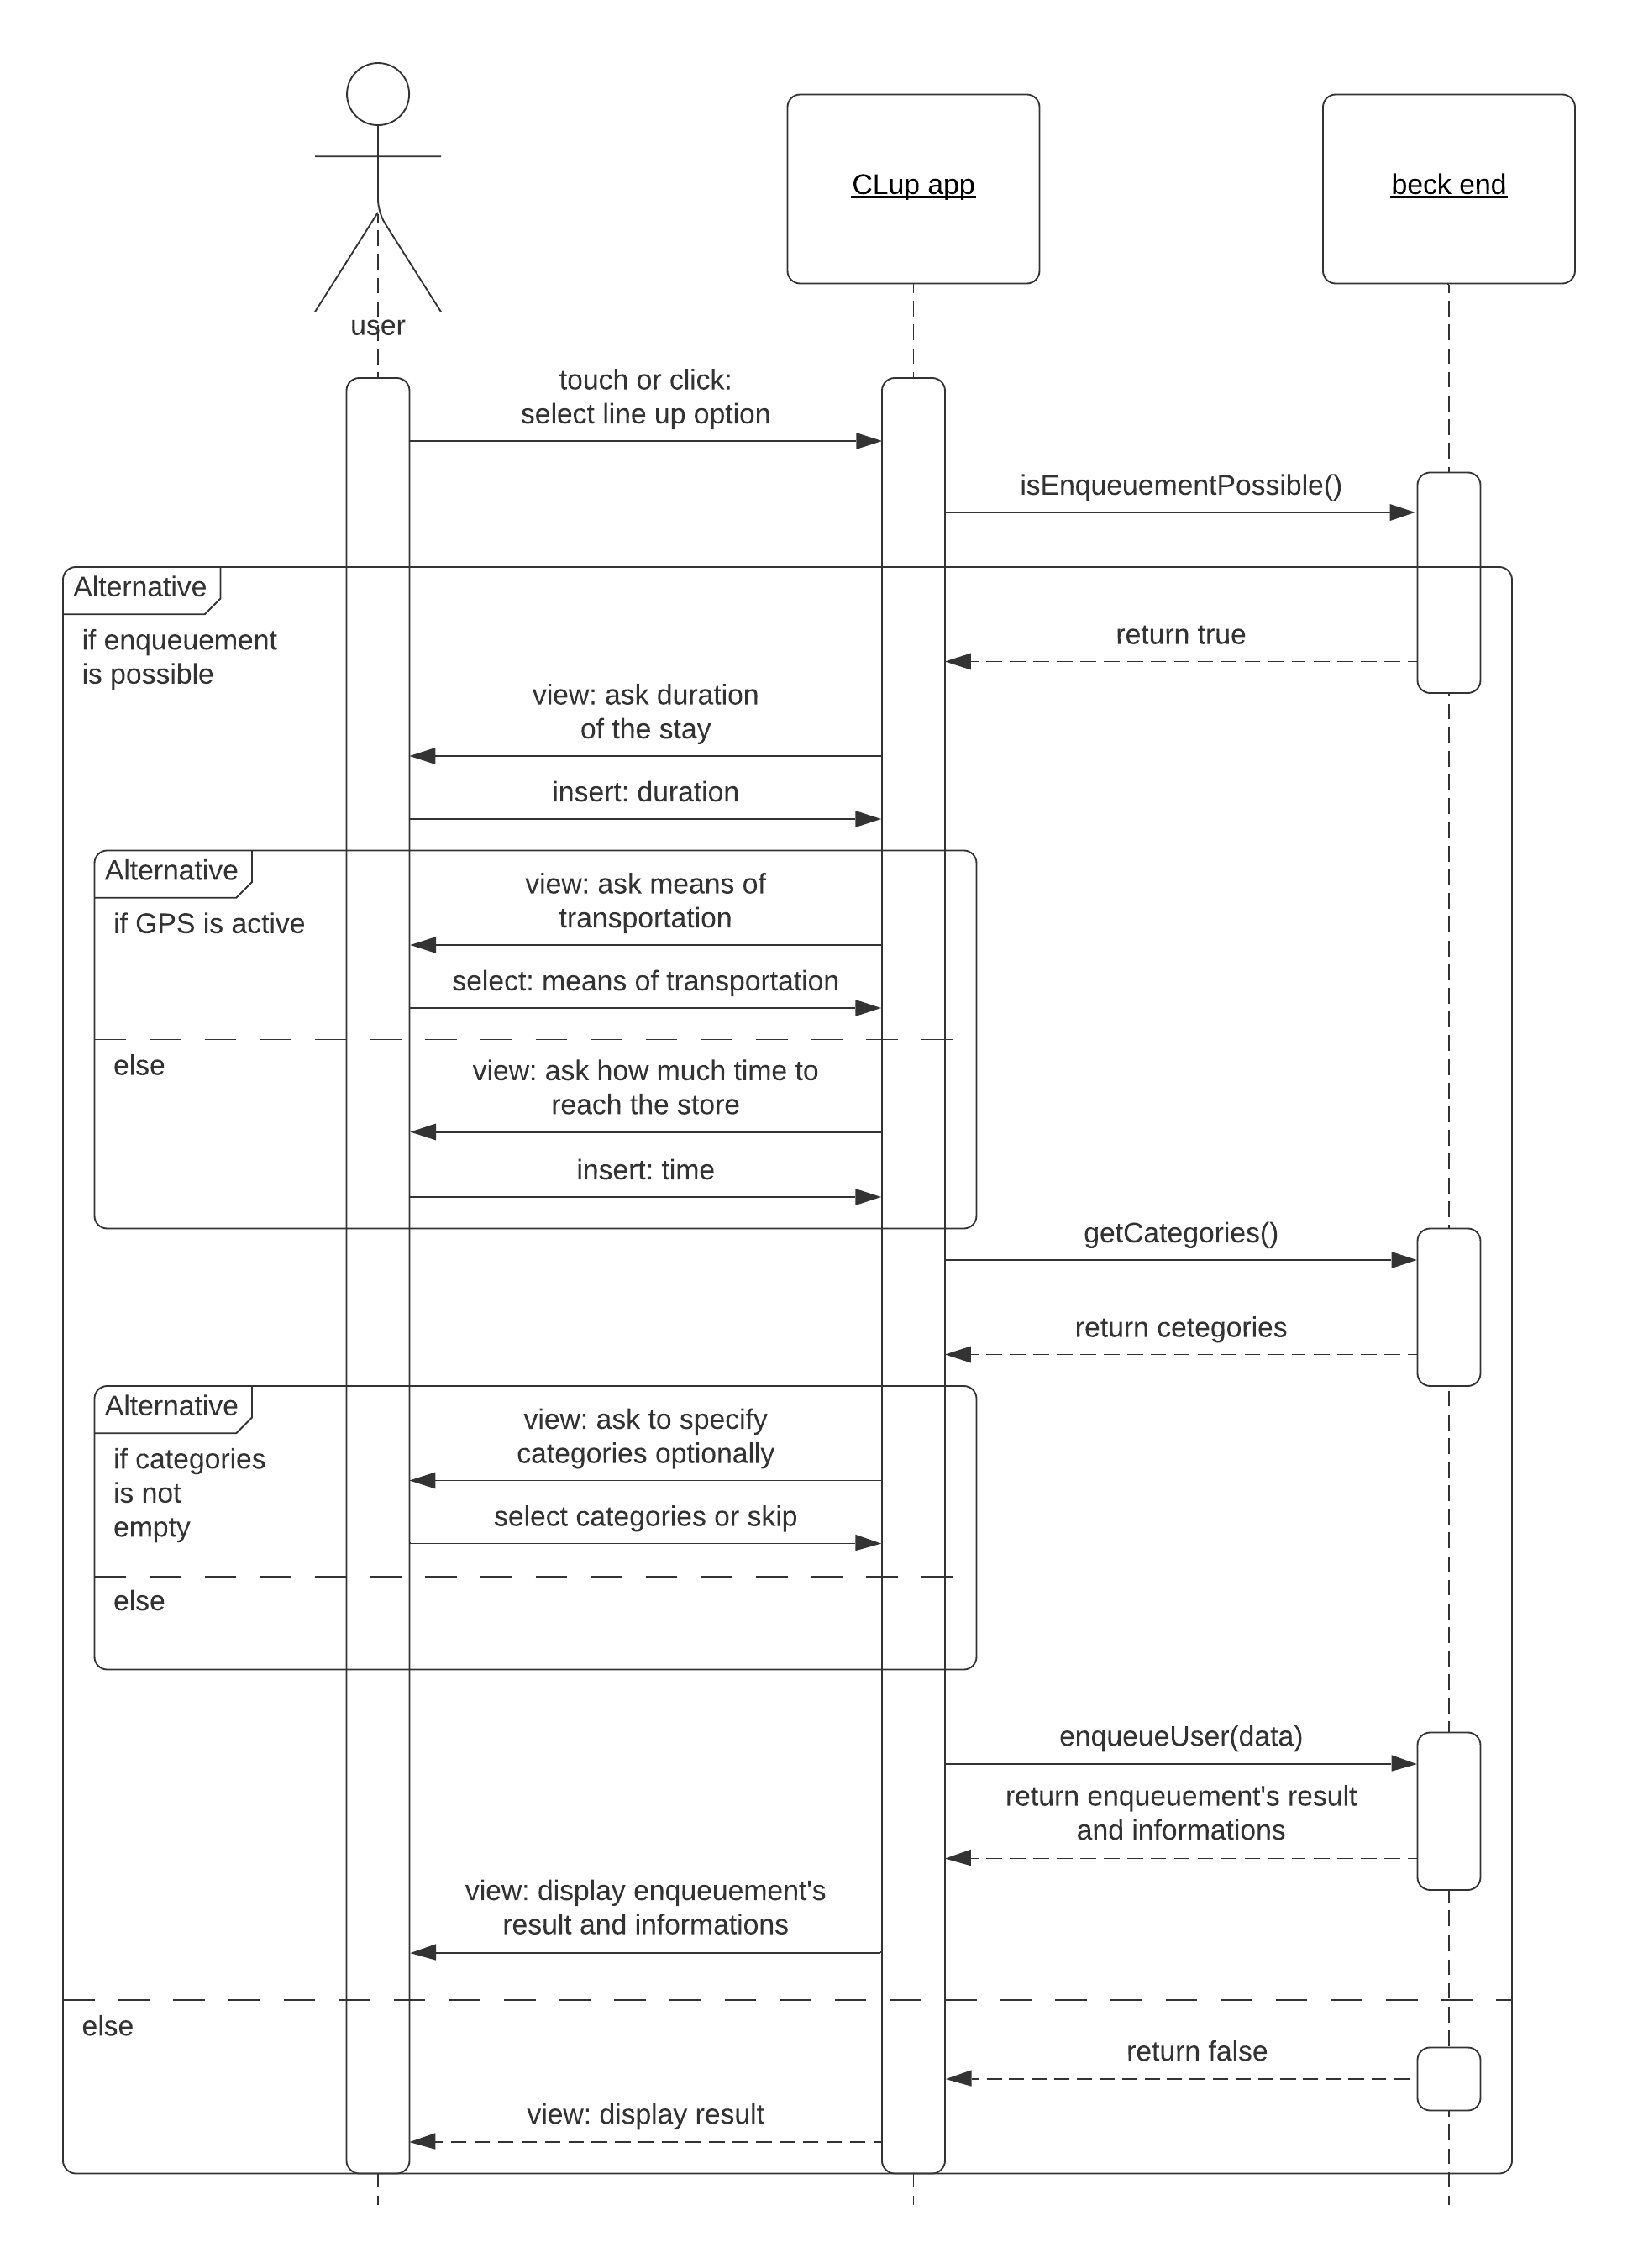
\includegraphics[width=\textwidth]{Images/sequencediagrams/UserlinesupSD.png}
    \caption{\label{fig:userlinesup}User searches a shop - sequence diagram}
\end{figure}

\begin{figure}[h!]
    \centering
    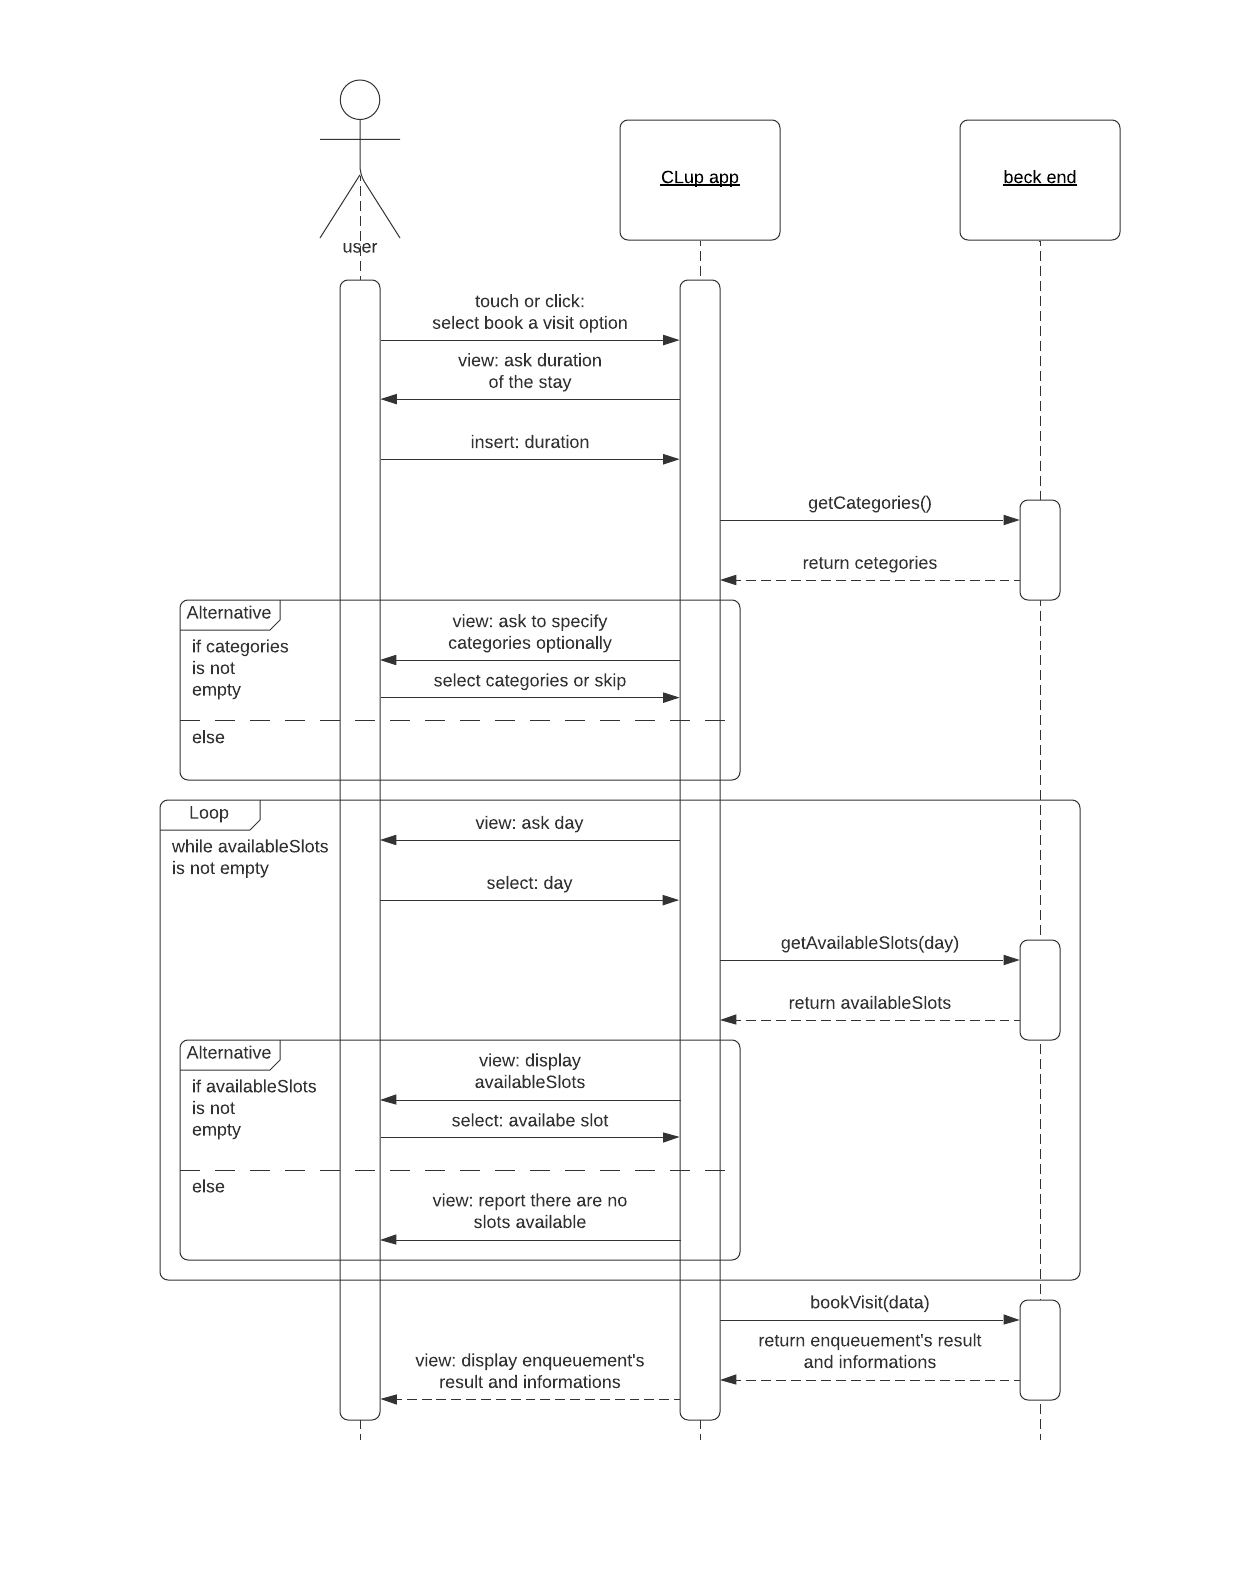
\includegraphics[width=\textwidth]{Images/sequencediagrams/UserbooksavisitSD.png}
    \caption{\label{fig:userbookavisit}User searches a shop - sequence diagram}
\end{figure}

\begin{figure}[h!]
    \centering
    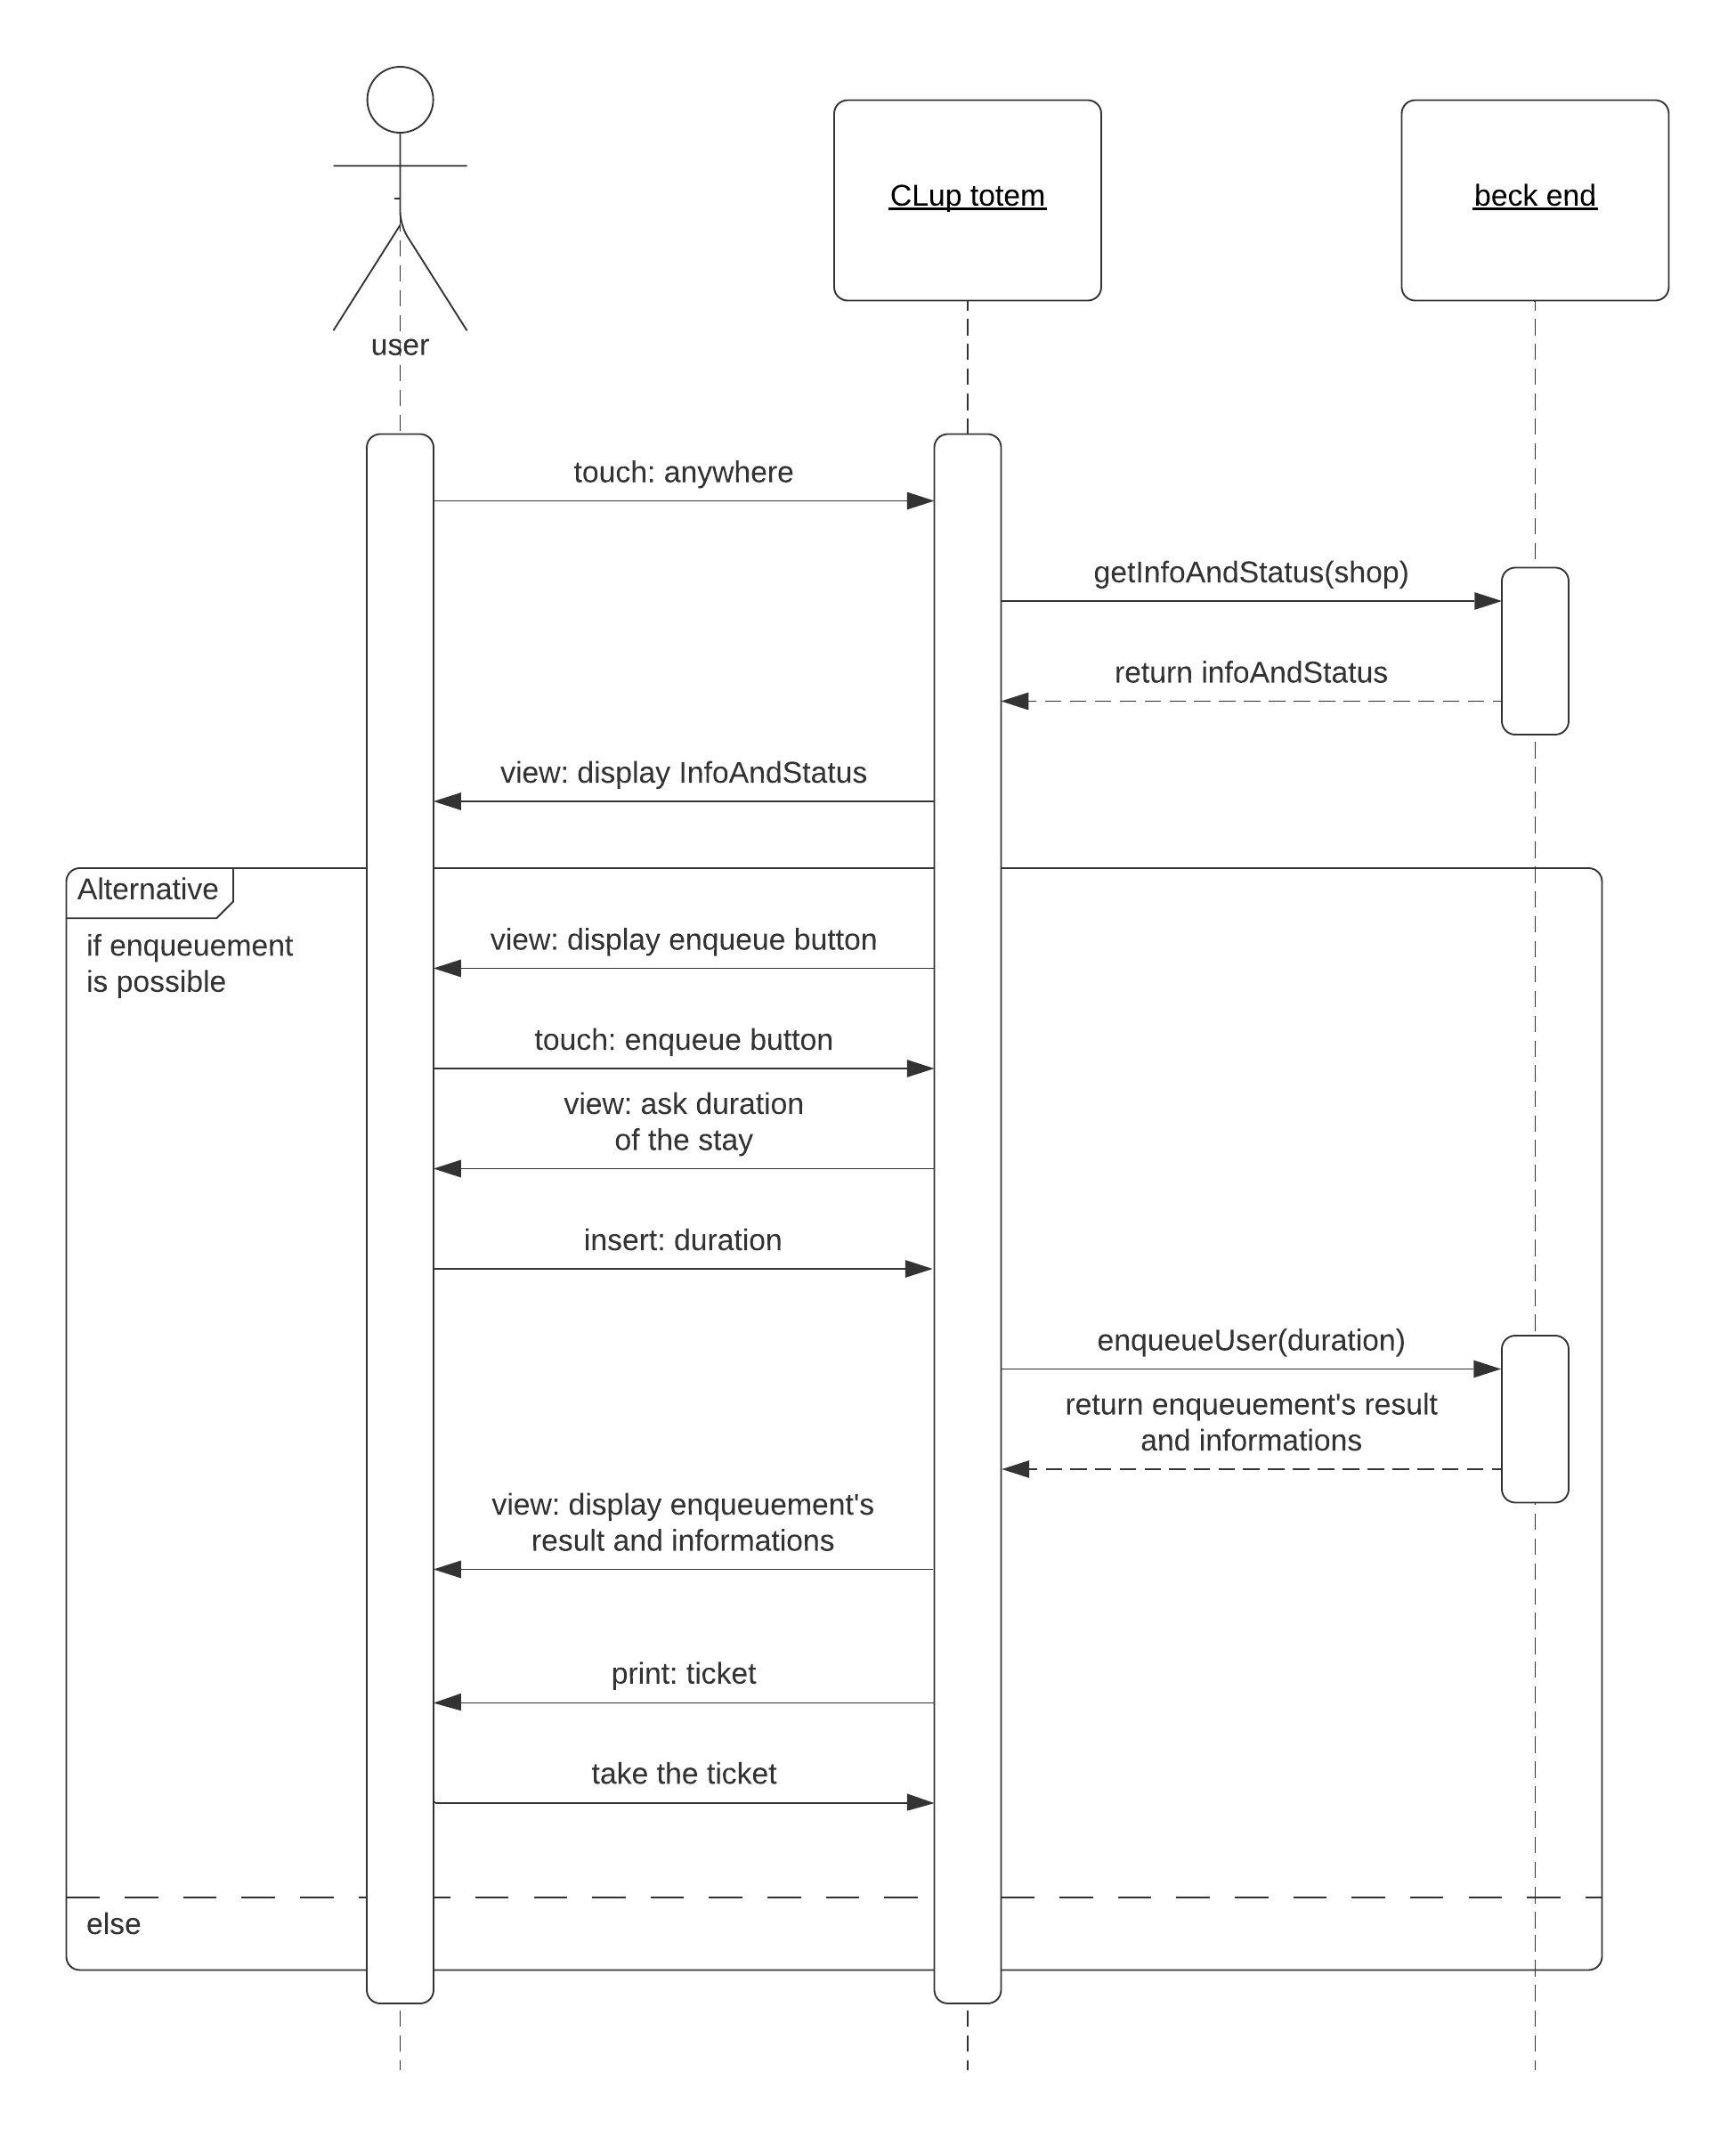
\includegraphics[width=\textwidth]{Images/sequencediagrams/CustomerlinesupSD.png}
    \caption{\label{fig:customerlinesup}User searches a shop - sequence diagram}
\end{figure}

\clearpage
\subsection{System structure}
\label{subsect:systemstructure}

\subsubsection{Functions}
\label{subsubsect:functionsstructure}

To better understand the overall interaction between all the functions and use cases described above, we present here a diagram that connects all the option an user can take.

\begin{figure}[h!]
    \centering
    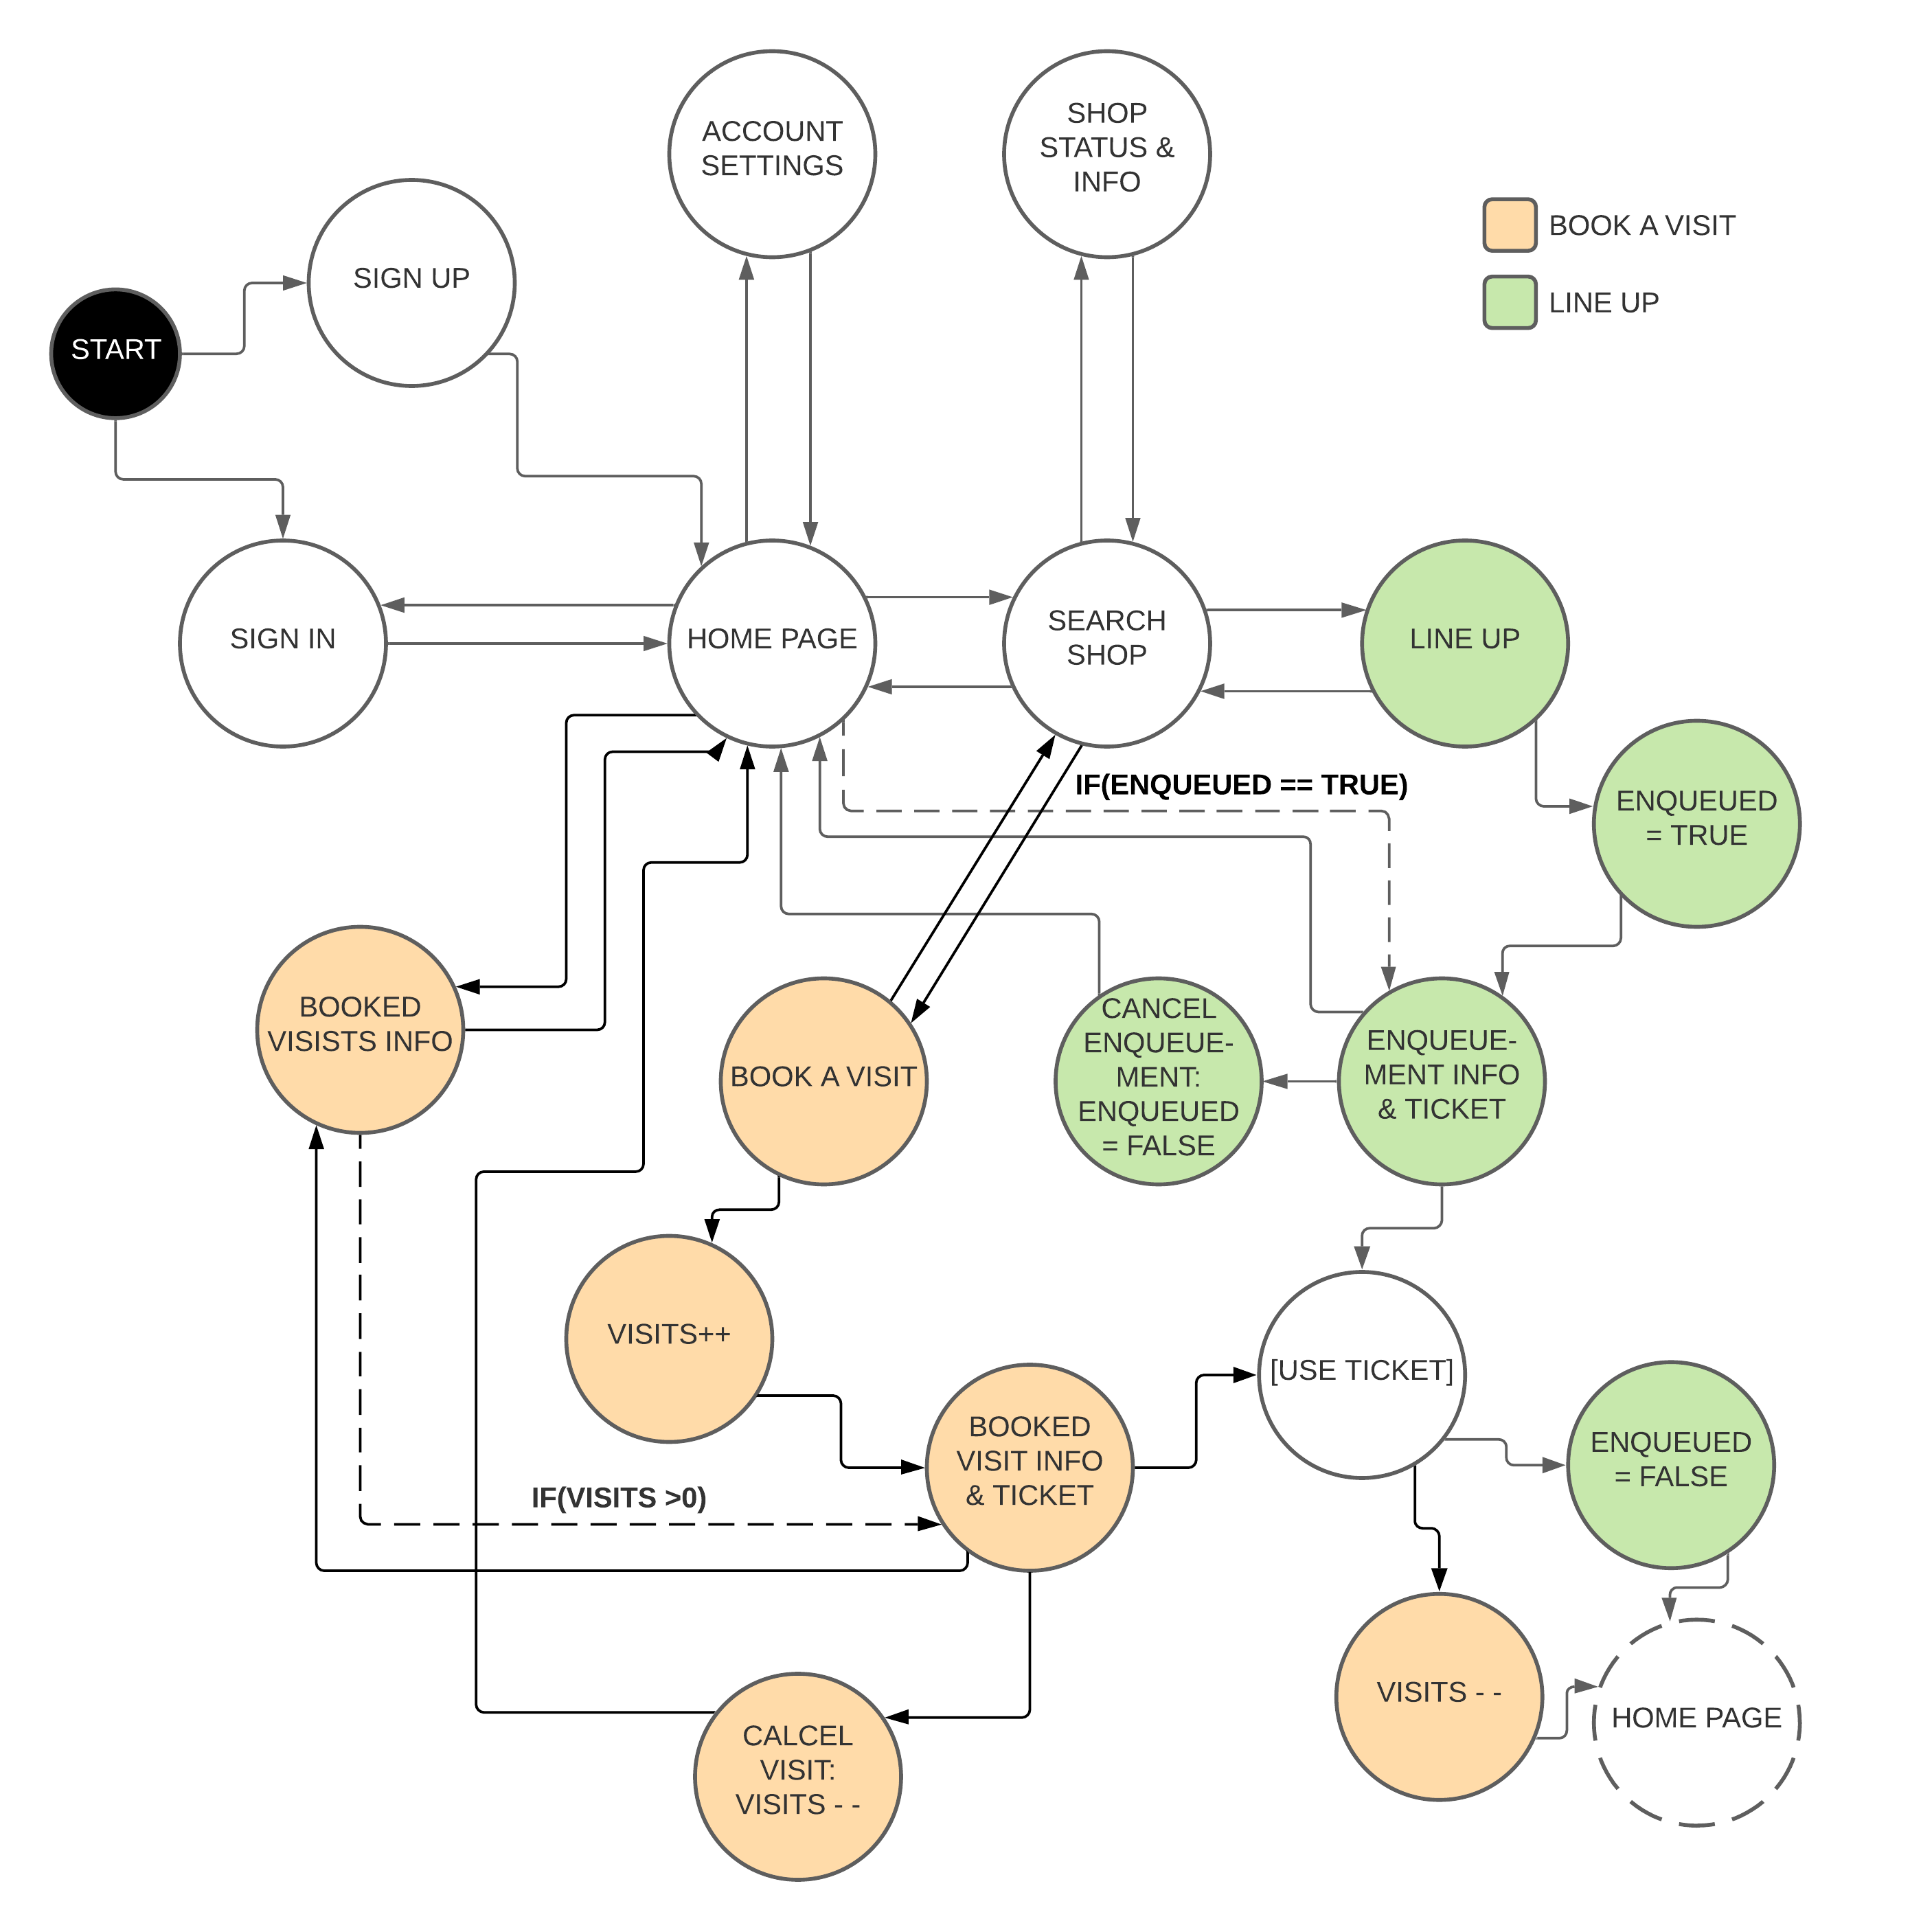
\includegraphics[width=\textwidth]{Images/statediagrams/userfunctions.png}
    \caption{\label{fig:userfunctions}{user's functions}}
\end{figure}

\FloatBarrier

Another aspect we want to highlight is the ticket system for booking visits and enqueuing users.

Even if booking a visit and enqueuing seems two totally different functions to the end user, for the system they are pretty much the same thing: an user who books a visit is like if he is enqueuing for a specific hour and day, and an user who decides to enqueue himself is like if he is booking a visit as soon as possible. 

Having specified these similarities, there are still some differences. A queue is a list that keeps track of user's turns to enter a shop and it is not a static structure, but it evolves throught time and through particular events, such as user's leaving queues or canceling booked visits and more. 
To handle queues, our system will constantly update and notify users of changes. Here we notice the only real difference between visit's ticket or queue's ticket: visit's ticket don't shift in time, queue's tickets do.

So once an user unqueues himself or books a visit the system generate a ticket and menages it according to the state diagram shown in the picture [\ref{fig:ticketlifecycle}]. A ticket can be in one of the following states:
\begin{itemize}[topsep=0pt]
    \item \textbf{valid ticket}: when a ticket is created it is always \textit{valid}, and that means that is waiting to be used to enter a shop.
    \item \textbf{in use ticket}: a ticket is \textit{in use} from the time it is used to enter the shop, to the time it is used to exit the shop.
    \item \textbf{used ticket}: an \textit{used} ticket is a ticket that has been successfully used to exit a shop. 
    \item \textbf{expired ticket}: \textit{expired} ticket is a ticket that can't be used to enter a shop because his turn has passed. This state could have been avoided by integrating it in the \textit{used} state, but in order to have a better understanding of the life's cycle of tickets we included it in here. 
\end{itemize}

\begin{figure}[h!]
    \centering
    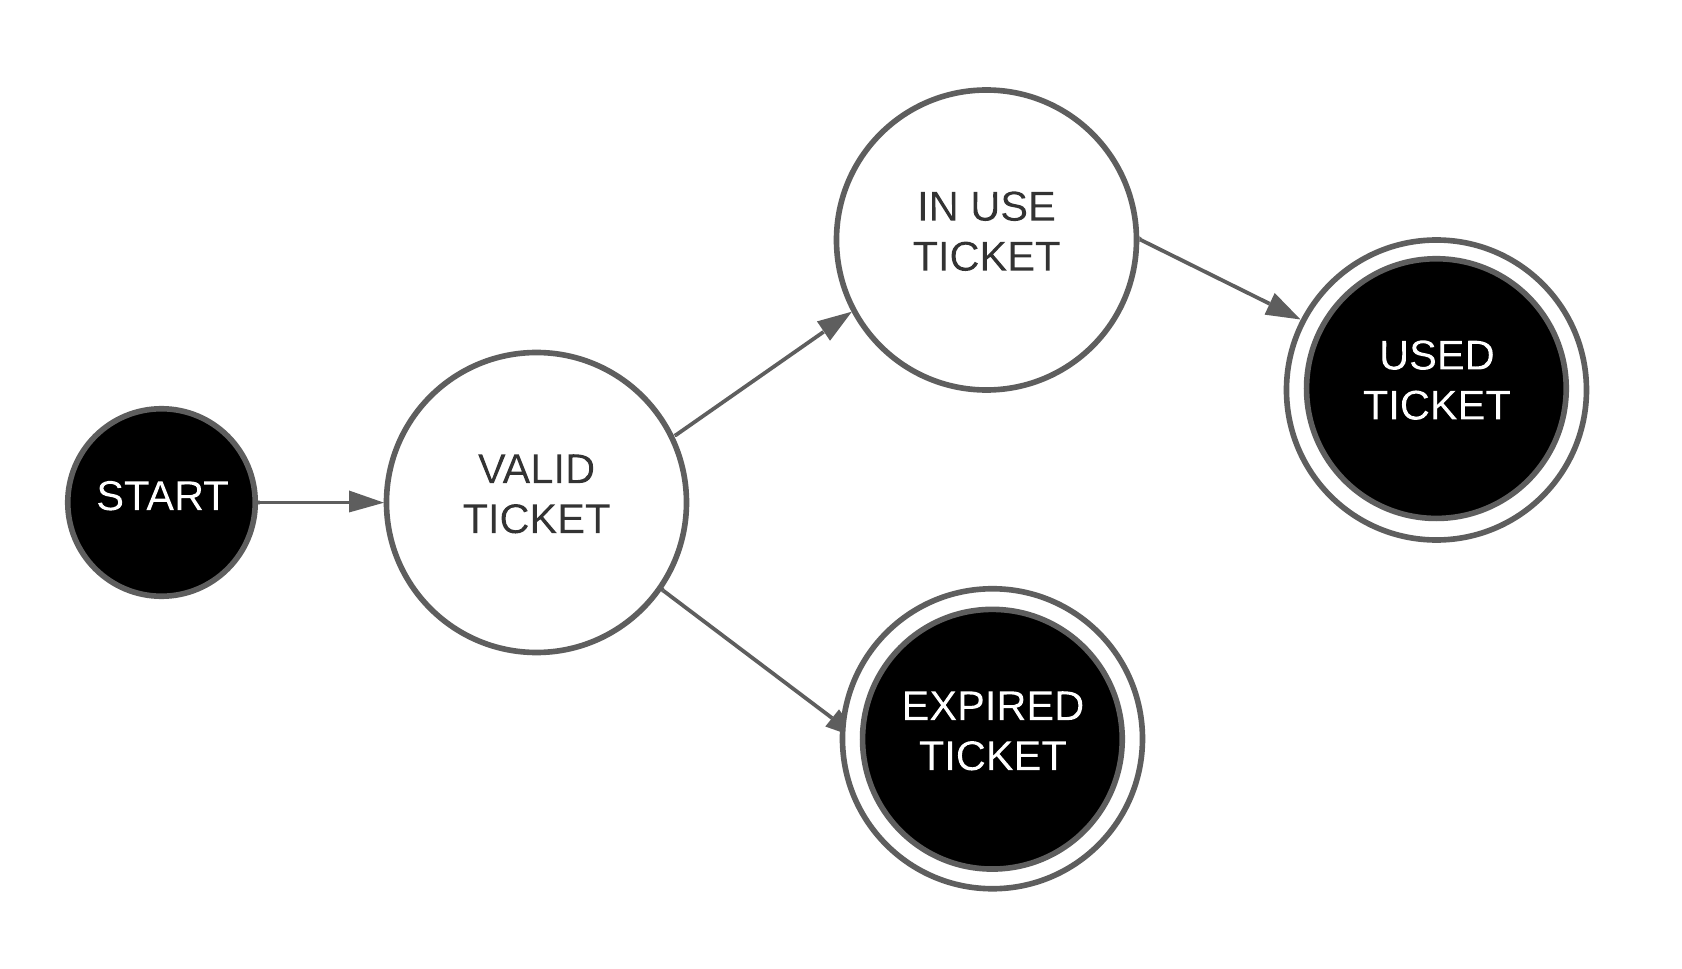
\includegraphics[height=6cm]{Images/statediagrams/ticketlifecycle.png}
    \caption{\label{fig:ticketlifecycle}State diagram: ticket's life cycle}
\end{figure}

\FloatBarrier

\subsubsection{Application model}
\label{subsubsect:applicationstructure}

In this section we want to present an early idea of an high-level abstraction of our application's structuree. To be noticed is that it is mainly modeled with focus on the data and their interaction.

TODO: UML + commento.